%% The following is a directive for TeXShop to indicate the main file
%%!TEX root = diss.tex

\chapter{A Mapping of 3D Reconstruction}
\label{ch:3DRecon_Mapping}
Most vision work focuses on developing algorithmic novelties, and as we have mentioned, very few investigate the rigorous conditions under which the algorithms themselves work. Thus, this knowledge is only known empirically, without a rigorous definition of the application domain or problem conditions. This relation between problem space and algorithms (termed as \textit{mapping}) is one of the key components of the interpreter, and is responsible for selecting one of the best possible algorithms based on described problem condition. This section builds upon the 3D description proposed in Chapter~\ref{ch:3DRecon_Desc}, and attempts to find the problem conditions surrounding each algorithm empirically. 

To achieve this goal, we need a dataset to evaluate the performance of each algorithm under varied problem conditions, which is not available since most 3D benchmarks, to the best of our knowledge, focus on one specific class of algorithms. For example, the Middlebury dataset targets MVS algorithms~\cite{seitz2006comparison}, and the `DiLiGenT' dataset targets Photometric Stereo algorithms~\cite{shi2016benchmark}. This makes such benchmarks only suitable for evaluation of within-category algorithms. Besides, there are no datasets with objects that cover a range of properties of materials and geometry. The reason for the lack of such a dataset is that it is practically impossible to change one property, \eg surface texture, material, and so on, while fixing others when creating a real-world dataset.

In response to these challenges, we use synthetic datasets created by phiyical-based rendering software (Blender), to evaluate the 3D reconstruction algorithms. Our dataset includes a collection of images of a scene under different materials and lighting conditions. The camera/projector's intrinsic and extrinsic parameters are computed directly from the configurations of the synthetic setup, and the ground truth, including the 3D model point cloud and normal map, are generated directly from Blender.

\section{Synthetic setup}
We use Blender's physical-based rendering engine, Cycles, to generate the synthetic datasets. For each technique, the configuration of the camera remains fixed. The image resolution is 1280$\times$720, with a focal length of $35mm$ or $1400pix$. The synthetic setups are shown in Table~\ref{tab:synth_setup}, and some example synthetic images generated using the setups are shown in Figure~\ref{fig:synth_setup}.
\begin{table}[!htbp]
\centering
\begin{tabular}{lll}
\toprule
Method & Hardware number & Arrangement\\
\midrule
MVS & 41 camera & 5 rings, each having 1, 8, 8, 12, 12 camera\\
PS & 1 camera+25 lights & 4 rings, each having 1, 8, 8, 8, 8 light sources\\
SL & 1 camera\&projector & baseline angle: $10^\circ$\\
\bottomrule
\end{tabular}
\caption{Summary of synthetic setups.}
\label{tab:synth_setup}
\end{table}

\begin{figure*}[!htbp]
\centering
\begin{tabular}{ll}
Texture & \raisebox{-.5\height}{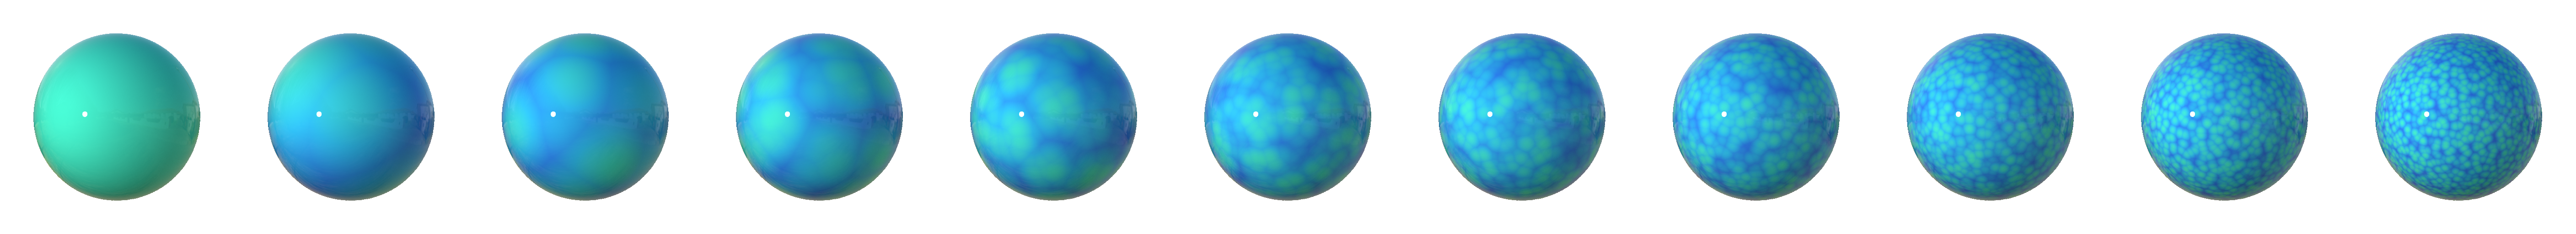
\includegraphics[width=0.8\textwidth]{img/mapping/setup/tex.png}}\\
Albedo & \raisebox{-.5\height}{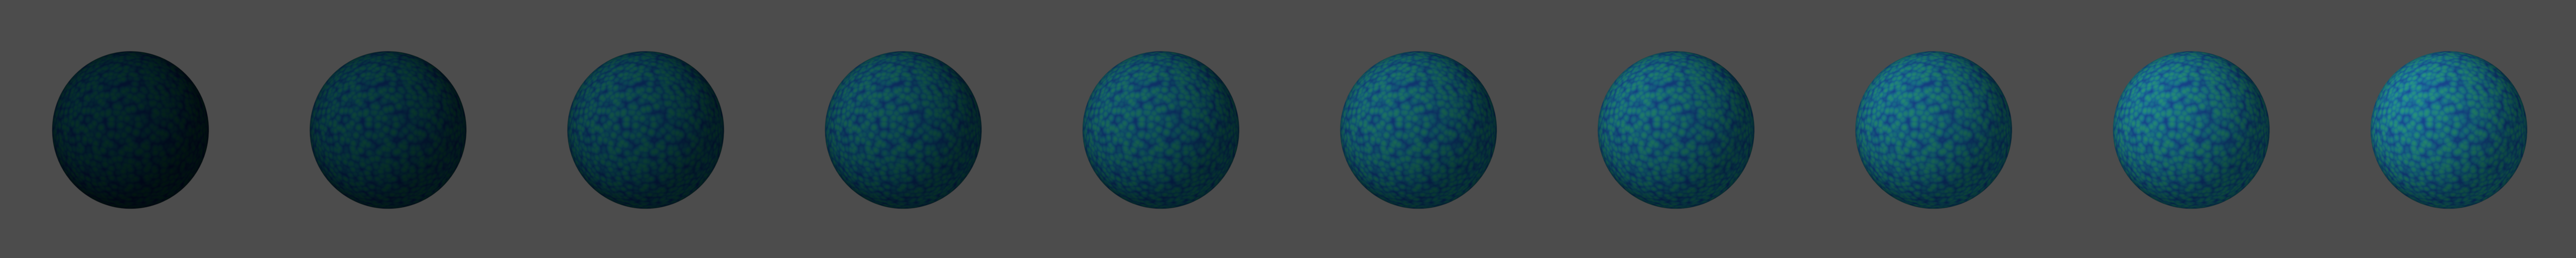
\includegraphics[width=0.8\textwidth]{img/mapping/setup/alb.png}}\\
Specular & \raisebox{-.5\height}{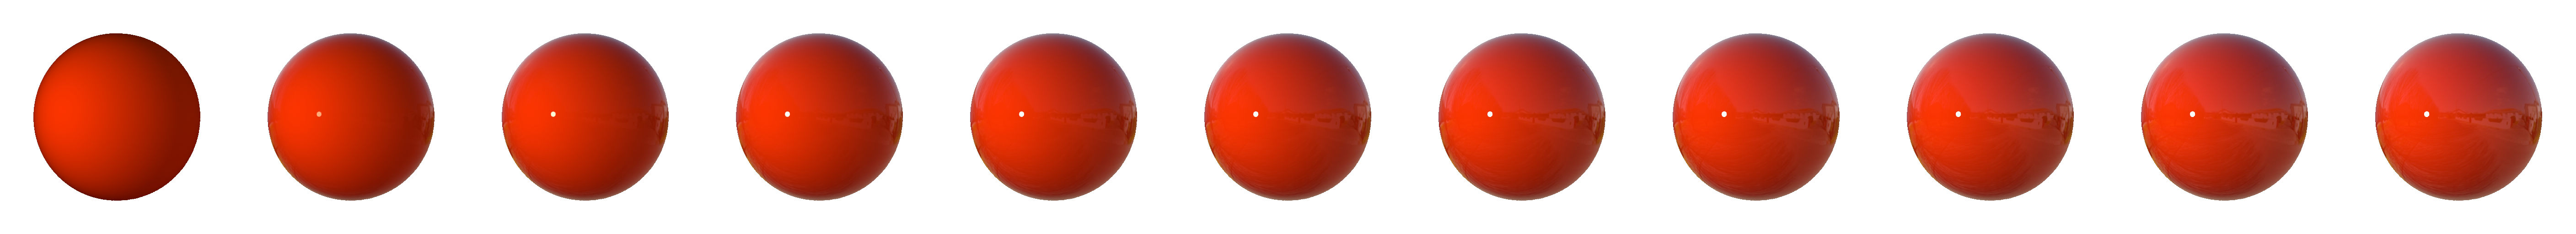
\includegraphics[width=0.8\textwidth]{img/mapping/setup/spec.png}}\\
Roughness & \raisebox{-.5\height}{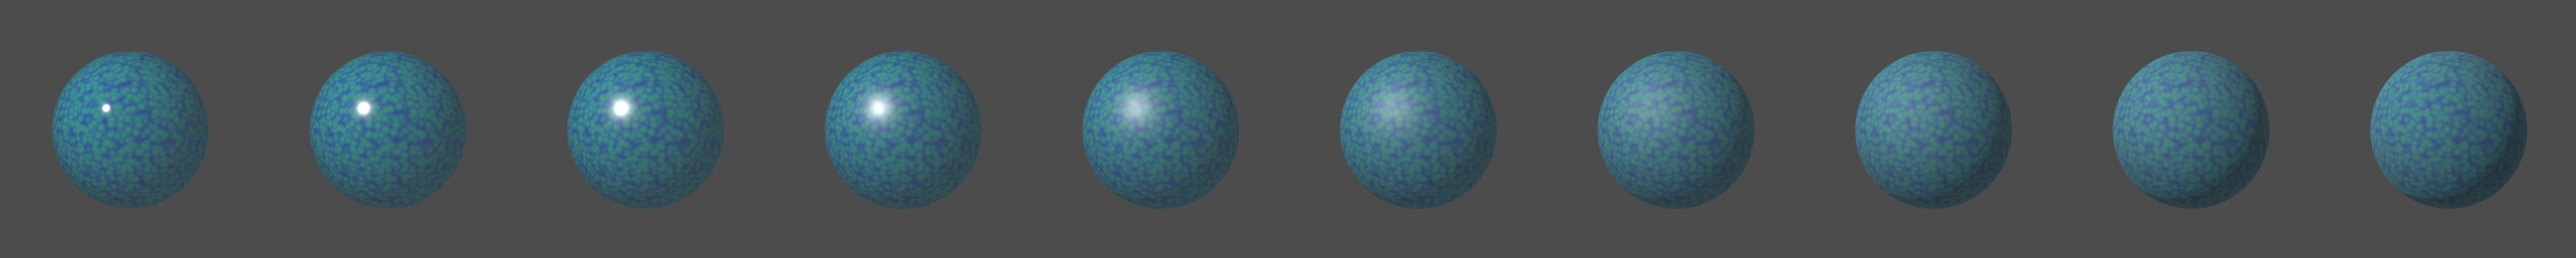
\includegraphics[width=0.8\textwidth]{img/mapping/setup/rough.png}}
\end{tabular}
\caption{Example synthetic images. The value of each property ranges from 0.1 to 1.}
\label{fig:synth_setup}
\end{figure*}

% For the Multi-View Stereo setup, there are five rings of cameras, of which the elevation angles are $15^\circ$, $30^\circ$, $45^\circ$, $60^\circ$, $90^\circ$. The between-angles of two neighbouring cameras are $30^\circ$, $30^\circ$, $45^\circ$, $45^\circ$, and $360^\circ$. Thus, there are in total $12+12+8+8+1=41$ cameras.

% For the Photometric Stereo setup, since increasing the number of images is only important up to a point, the experimental results showed that most algorithms reaches their optimum when 15 images are used~\cite{Berkiten:2016:ARB}. To strike a balance between algorithm performance and rendering time, we use 25 light sources, which are distributed on four rings with elevation angle of $90^\circ$, $85^\circ$, $60^\circ$, and $45^\circ$. The azimuth angle between two neighbouring light sources is $45^\circ$. Thus, the total number of images is $1+8*3=25$.

% For the Structured Light setup, the baseline angle between the camera and the projector is $10^\circ$. The resolution of the projector is $1024\times768$, thus 10 Gray code patterns are needed. To counter the effect of inter-reflection, each pattern and its inverse are projected, which descreases sensitivity to scattered light. Two additional image with lights on and off are generated to help the decoding process. Thus the total number of images is $(10+10)*2+2=42$.
% \begin{figure}[!htbp]
% \centering
% \begin{tabular}{ccc}
% 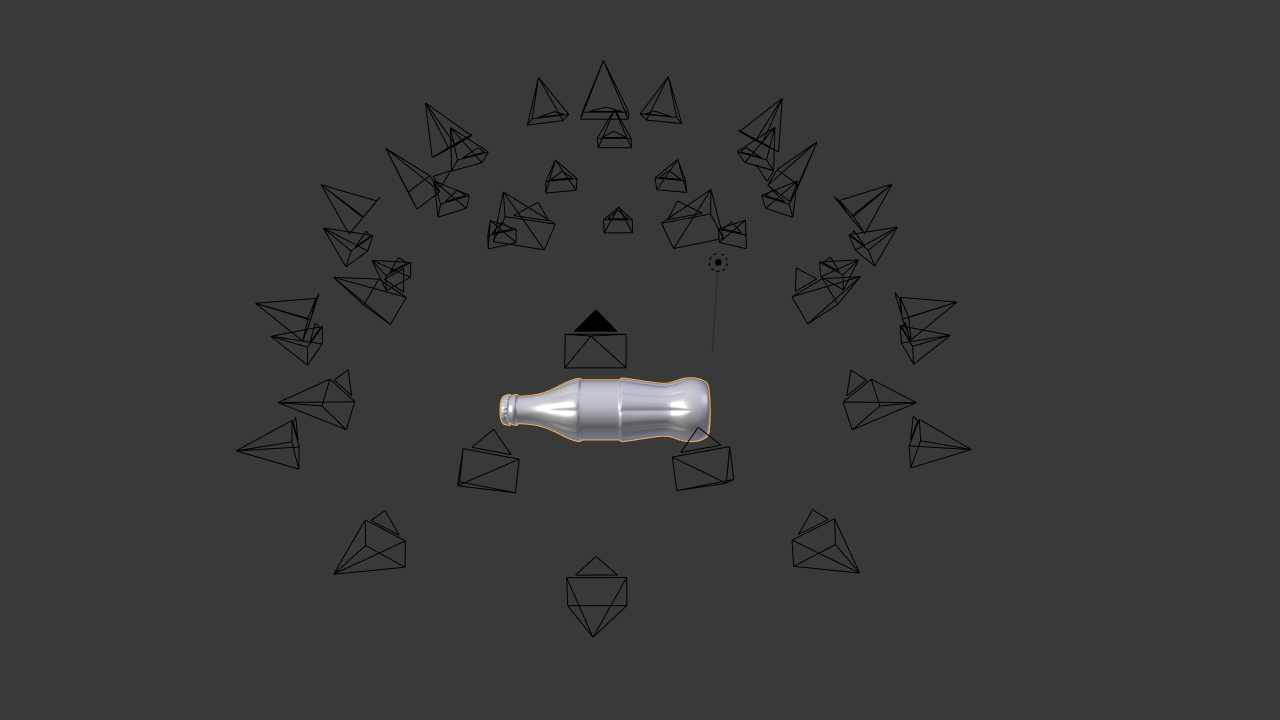
\includegraphics[width=0.3\textwidth]{mapping/setup/mvs_setup} &
% 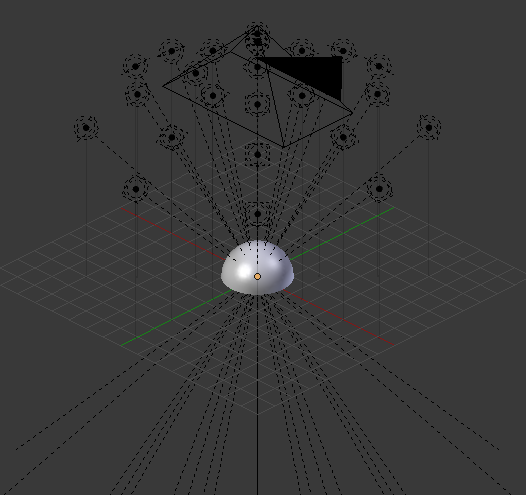
\includegraphics[width=0.3\textwidth]{mapping/setup/ps_setup} &
% 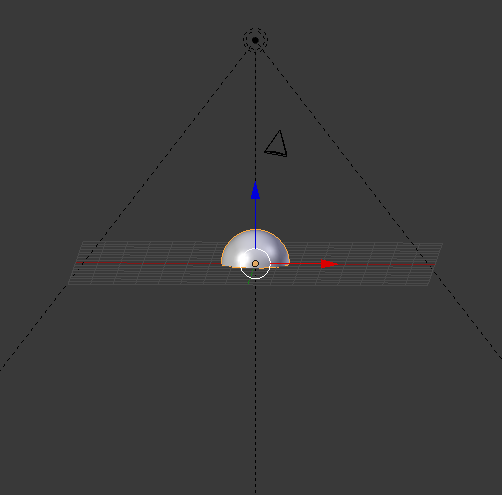
\includegraphics[width=0.3\textwidth]{mapping/setup/sl_setup}\\
% MVS & PS & SL\\
% \end{tabular}
% \caption{Setups of the syntheic dataset}
% \label{fig:setup}
% \end{figure}

% \section{Structure of Datasets}
% All synthetic datasets used in this thesis share the similar structure, as shown in Figure~\ref{fig:dataset_structure}. \textit{Prop Comb} represents one combination of properties, which consists of no less than two properties. For instance, \textit{texture and albedo}, or \textit{albedo, and specularity}. Note that the diretory structure of PS and SL is the same as that of MVS.
% Due to the number of properties and levels for each property, it would be unrealistic to render all their combinations. For instance, if there are $N$ properties and each is discretized into $L$ levels, the number of different combinations is $L^N$, and for each combination, there are in total $41+25+42=108$ images to render. Therefore, we take another approach: 1) we investigate the \textit{effective problem domain} which consists of only the \textit{effective} and \textit{dependent} properties; 2) we generate synthetic images for the \textit{effective} and \textit{dependent} properties and all of their combinations. The structure of the dataset is as follows:
% \begin{figure}[!htbp]
% \centering
% 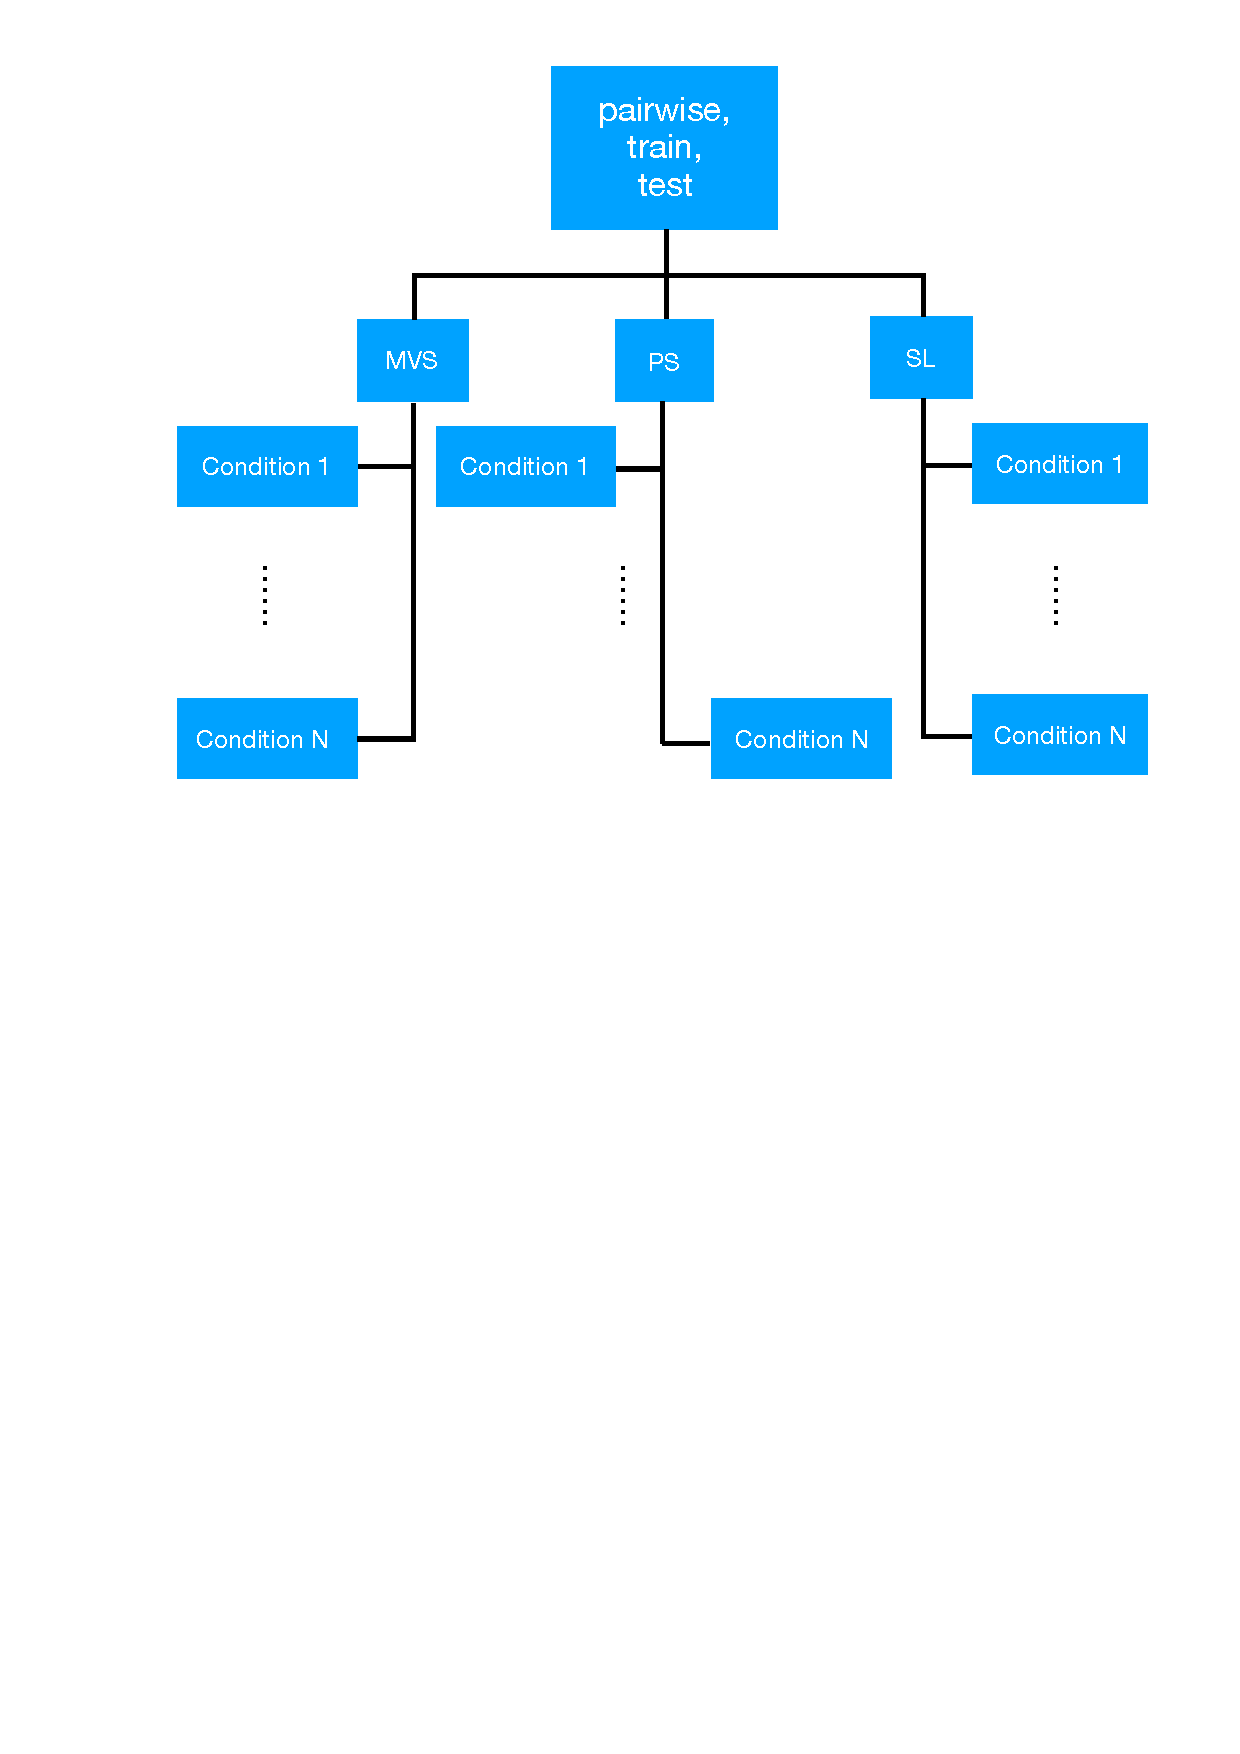
\includegraphics[width=0.6\textwidth]{mapping/dataset_structure}
% \caption{Structure of the synthetic dataset.}
% \label{fig:dataset_structure}
% \end{figure}

\section{Selected and baseline methods}
We have selected one representative algorithm from three major classes of algorithms presented in Chapter~\ref{ch:3DRecon_ProbSpace}: the PMVS proposed in~\cite{furukawa2010accurate}, the example-based Photometric Stereo proposed in~\cite{hertzmann2005example}, and the Gray-code Structured Light technique. See Table~\ref{tab:selected_algos} for a summary of the selected algorithms. The current implementation of SL projects both column and row patterns, and depth values are computed using these two kinds of patterns individually. A depth consistency step is performed to reject erroneous triangulations.
\begin{table}[!htbp]
\centering
\begin{tabular}{l|l}
\toprule
Technique & Summary\\
\midrule
PMVS & Patch-based, seed points propagation MVS.\\
EPS & Example-based Photometric Stereo.\\
GSL & Gray code Structured Light technique.\\
\midrule
VH & Volumetric Visual Hull.\\
LLS-PS & Linear least squares Photometric Stereo.\\
\bottomrule
\end{tabular}
\caption{Summary of the selected and baseline algorithms for the interface, and the corresponding working conditions in theory.}
\label{tab:selected_algos}
\end{table}

% \section{Baseline}
% \begin{table}[!htbp]
% \centering
% \begin{tabular}{c|c|c|c|c}
% \toprule
% Technique & Texture & Albedeo & Specular & Roughness\\
% \midrule
% \multicolumn{5}{l}{VH: volumetric Visual Hull}\\
% \midrule
% VH & - & - & - & -\\
% \midrule
% \multicolumn{5}{l}{LLS-PS: linear least squares Photometric Stereo.}\\
% \midrule
% LLS-PS & - & High & Low & High\\
% \bottomrule
% \end{tabular}
% \caption{Summary of the baseline algorithms for the framework, and the corresponding working conditions in theory.}
% \label{tab:selected_baseline_algos}
% \end{table}
We use two baseline approaches to compare our results: Visual Hull and a simple linear least squares based Photometric Stereo (LLS-PS). We use Visual Hull since it works relatively well as long as the silhouette of the object can be reliably extracted, thus being insensitive to material properties. In addition, the true scene is always enclosed by the reconstruction result, so the outcome is always predictable. We use LLS-PS to evaluate Photometric Stereo algorithms. However, there is currently no such PS algorithms that work reasonably well under a variety of conditions. Thus, we run this baseline algorithm under the optimal condition to ensure a best possible result.

\section{Quantitative measures}
We use the metrics proposed in \cite{seitz2006comparison} to evaluate MVS and SL algorithms. More specifically, we compute the accuracy and completeness of the reconstruction. For accuracy, the distance between the points in the reconstruction $R$ and the nearest points on ground truth $G$ is computed, and the distance $d$ such that $X\%$ of the points on $R$ are within distance $d$ of $G$ is considered as accuracy. A reasonable $d$ value is between $[3, 5]mm$, and $X$ is set as $95$. The lower the accuracy value, the better the reconstruction result. For completeness, we compute the distance from $G$ to $R$. Intuitively, points on $G$ are not ``covered'' if no suitable nearest points on $R$ are found. A more practical approach computes the fraction of points of $G$ that are within an allowable distance $d$ of $R$. Note that as the accuracy improves, the ``accuracy value'' goes down, whereas as the completeness improves, the ``completeness value'' goes up.

For photometric stereo, depth information is lost since only one viewpoint is used. Thus, the previous metrics are not applicable. Here we employ another evaluation criteria that is widely adopted, which is based on the statistics of angular error. For each pixel, the angular error is calculated as the angle between the estimated and ground truth normal, \ie $arccos$($n_g^T n$), where $n_g$ and $n$ are the ground truth and estimated normals respectively. In addition to the mean angular error, we also calculate the standard deviation, minimum, maximum, median, first quartile, and third quartile of angular errors for each estimated normal map.

% \subsection{Criteria}
% We compare the quantitative measures of a result to those of the baseline method to determine if it is a successful reconstruction. The following rules determines if a specific algorithm returns a successful reconstruction.

% For results of MVS and SL, we use both accuracy and completeness to determine if a result is successful. However, methods that return accurate results do not necessarily produce complete results. Thus, we consider a result successful if the accuracy is better while completeness is comparable to that of the baseline.

% For results of PS algorithms, we use the central value, variation, and skewness of angular error to determine if a result if successful. The rationale is explained below:

% \subsubsection{Measures of Central Tendency}
% Mean and median are both valid measures of central tendency, but as the skewness increases, the mean is dragged in the direction of the skew. As a result, the median is generally considered to be a better representative of the central location of the data. The more skewed the distribution, the greater the difference between the median and mean, and the greater the emphasis should be placed on using the median as opposed to the mean.

% \subsubsection{Variation}
% The variation of the angular error is measured by both \textit{interquatile range} ($Q_3 - Q_1$) and \textit{standard deviation} ($std$).
  
% \subsubsection{Skewness (right/positive-skewness)}
% The normal estimation becomes worse as the difference between mean and median increases. This can be explained as follows: assuming the angular error follows a Gaussian distrubtion, then mean and median are close when the normals are reliably estimated. However, if normals are poorly recovered, the mean would increase since larger angular errors exist, while the median would change far less since only a small amount of pixels are poorly estimated. Thus, the difference between mean and median is a good indicator of the quality of normal estimation.

\section{Effective Problem Domain (EPD)}
The greatest challenge in constructing a mapping from problem space to algorithms is the large variations in shapes and material properties, which results in a problem space that is too large to cope with. Suppose there are $N$ properties, each with $L$ discrete levels, then there are in total $L^N$ different problem conditions. Thus, the first step, discussed in Section~\ref{sec:mvs_epd},~\ref{sec:ps_epd},~\ref{sec:sl_epd}, is to reduce the dimensions of problem space by establishing the \textit{effective problem domain} $\text{EPD}=\text{set(}p_i^j\text{)}$, where $i\in\{0, ..., L-1\}$, and $j\in \{0, ..., N-1\}$, which consists of only effective properties. Then, Section~\ref{sec:mvs_training},~\ref{sec:ps_training},~\ref{sec:sl_training} evaluate performance of selected algorithms within the corresponding EPD.

A naive way of finding the \textit{effective properties} would be evaluating algorithmic performance by changing one property at a time. However, this approach ignores the dependency between properties, \ie the effect of property \textit{A} might be insignificant when property \textit{B} is absent. Thus, we investigate the pairwise relation between any two properties, thus two properties are chosen while the rest are fixed, the configurations of the problem conditions are shown in Table~\ref{tab:pairwise_prob_cond}

\begin{table}[!htbp]
  \centering
  \begin{tabular}{l*{4}{c}}
  \hline
  \textbf{Cond.} & Texture & Albedo & Specular & Roughness\\
  \hline
  \textbf{(a)} & [0.2, 0.8] & [0.2, 0.8] & 0.0 & 0.0\\
  \textbf{(b)} & [0.2, 0.8] & 0.8 & [0.2, 0.8] & 0.0\\
  \textbf{(c)} & [0.2, 0.8] & 0.8 & 0.0 & [0.2, 0.8]\\
  \textbf{(d)} & 0.8 & [0.2, 0.8] & [0.2, 0.8] & 0.0\\
  \textbf{(e)} & 0.8 & [0.2, 0.8] & 0.0 & [0.2, 0.8]\\
  \textbf{(f)} & 0.8 & 0.8 & [0.2, 0.8] & [0.2, 0.8]\\
  \hline
  \end{tabular}
  \caption{Problem conditions for establishing the \textit{effective problem domain} of all selected algorithms. For instance, cond. (a) considers texture and albedo while specularity and roughness are fixed. The value of both varying properties range from 0.2 to 0.8.}
  \label{tab:pairwise_prob_cond}
\end{table}

\subsection{EPD: PMVS}
\label{sec:mvs_epd}
We investigate the impact of each property on the performance of PMVS in terms of accuracy and completeness under varied combinations of properties. The settings of these properties are listed in Table~\ref{tab:pairwise_prob_cond}.

\begin{sidewaysfigure}[!htbp]
\begin{tabular}{ccc}
\includegraphics[width=0.3\textwidth]{mapping/depend_check/mvs_tex_alb}&
\includegraphics[width=0.3\textwidth]{mapping/depend_check/mvs_tex_spec}&
\includegraphics[width=0.3\textwidth]{mapping/depend_check/mvs_tex_rough}\\
(a) & (b) & (c)\\
\includegraphics[width=0.3\textwidth]{mapping/depend_check/mvs_alb_spec}&
\includegraphics[width=0.3\textwidth]{mapping/depend_check/mvs_alb_rough}&
\includegraphics[width=0.3\textwidth]{mapping/depend_check/mvs_spec_rough}\\
(d) & (e) & (f)\\
\end{tabular}
\caption{Performance of PMVS under six pairwise conditions. For instance, (a) shows the performance under changing \textit{texture} and \textit{albedo} values, while the others are fixed. The property values are set based on settings in Table~\ref{tab:mvs_depend_check_params}.}
\label{fig:mvs_depend_check}
\end{sidewaysfigure}

\textbf{(a) Texture and Albedo} 
texture has a positive effect on the reconstruction in terms of accuracy and completeness, while the effect of albedo is negligible.

\textbf{(b) Texture and Specularity} 
specularity has a negative effect on both the accuracy and completeness of the reconstruction. However, the level of impact varies as the texture varies. More specifically, the effect of specularity is more substantial on a less textured surface, as shown in Figure~\ref{fig:mvs_depend_check} (b). This can be explained as follows: the specular lobe can only be observed by cameras positioned and oriented towards the specular lobe, such as camera $V_2$ shown in Figure~\ref{fig:mvs_spec} (a) and (c). Cameras positioned otherwise would observe the true surface, such as camera $V_1$ shown in Figure~\ref{fig:mvs_spec} (a) and (b). The algorithm would then exploit the texture information provided by views like $V_1$, and thus would be able to reconstruct a specular surface.
\begin{figure}[!htbp]
\begin{tabular}{ccc}
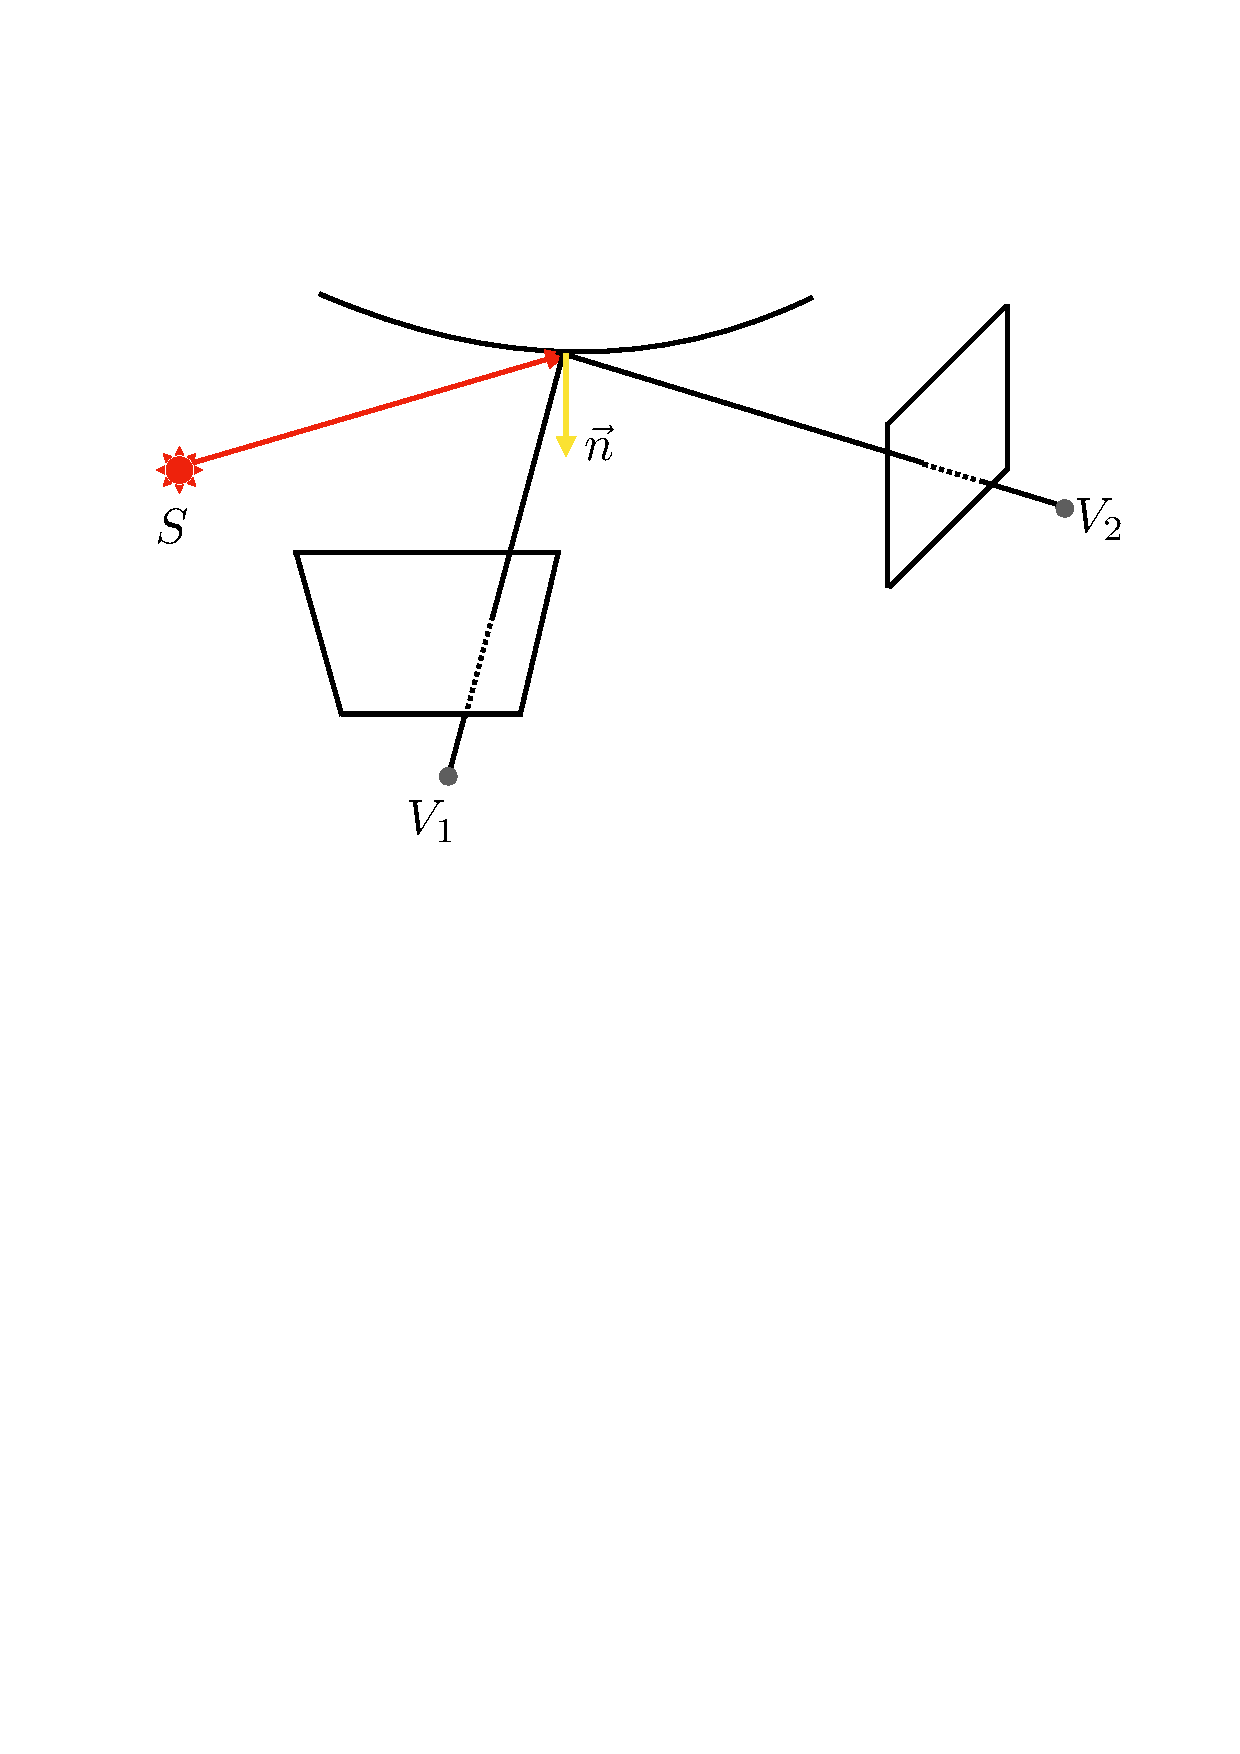
\includegraphics[width=0.33\textwidth]{mapping/mvs_spec/mvs_spec}&
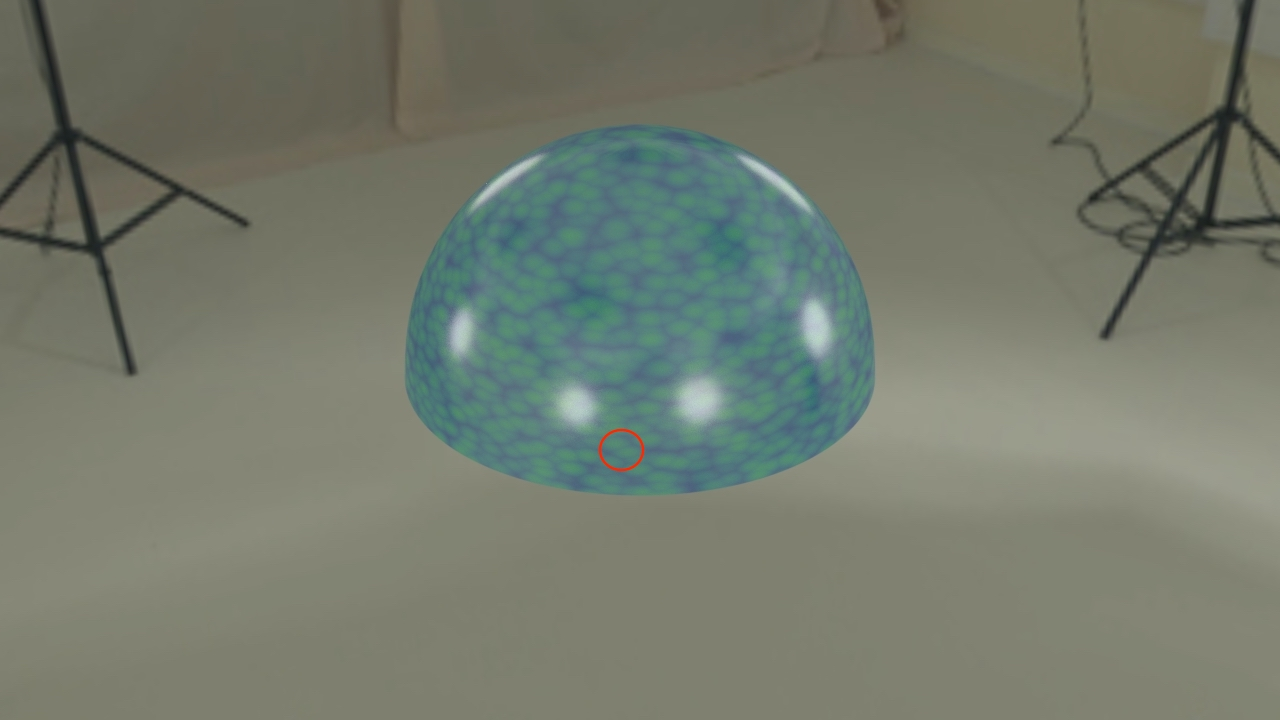
\includegraphics[width=0.33\textwidth]{mapping/mvs_spec/mvs_spec_01}&
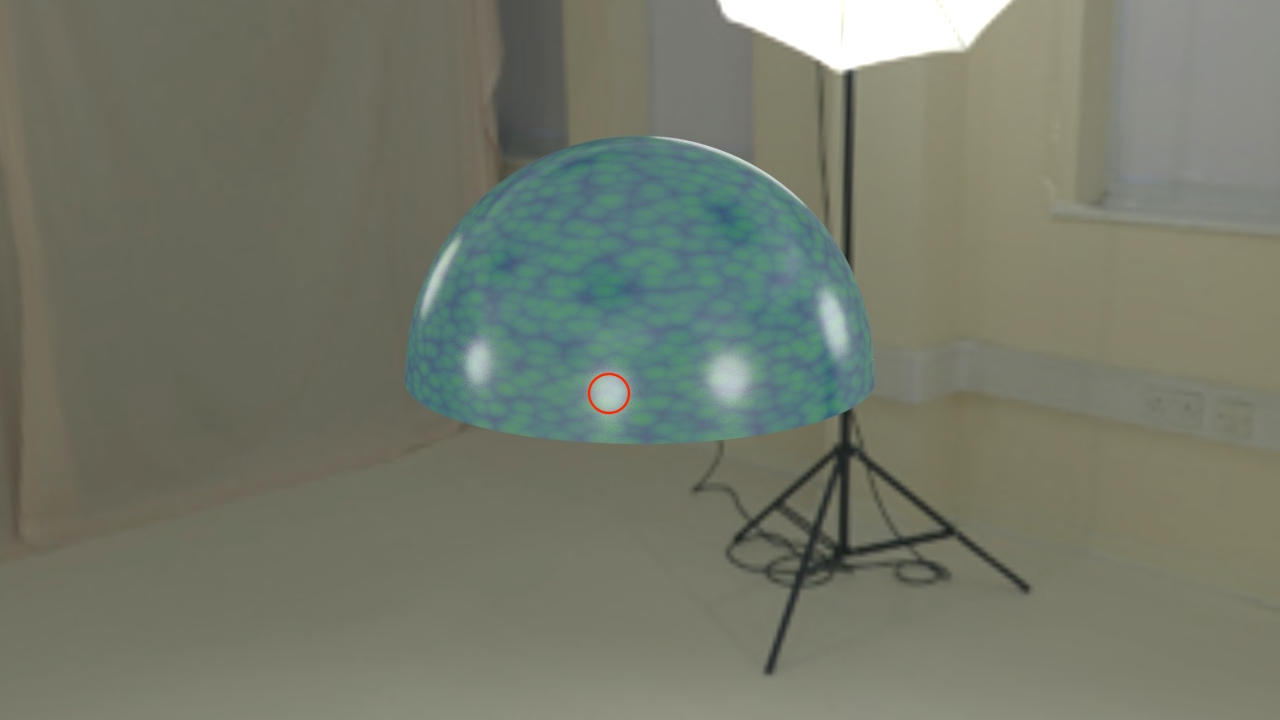
\includegraphics[width=0.33\textwidth]{mapping/mvs_spec/mvs_spec_00}\\
(a) Image formation & (b) $V_1$ & (c) $V_2$\\
\end{tabular}
\caption{(a) shows the reflection of light off a specular surface. $V_1$ received the diffuse component while $V_2$ receives the specular component. (b), (c) shows the images observed from these two views. The specular area (red circle) observed in $V_2$ is visible in $V_1$.}
\label{fig:mvs_spec}
\end{figure}

\textbf{(c) Texture and Roughness} 
roughness doesn't have a significant effect on the results.

\textbf{(d) Albedo and Specular} 
albedo has a positive effect whereas specular has a negative effect on the reconstruction. Furthermore, the positive effect of albedo is more significant on a higher specular surface while the negative effect of specular is far more substantial on a lower albedo surface. This can be explained as follows: according to the energy conservation law, as the specular component increases, the diffuse component decreases, resulting in a less discernible diffuse area. See Figure~\ref{fig:mvs_alb_spec} (a)-(c). Increasing the diffuse albedo can counteract the effect of specularity and make the texture visible again. See Figure~\ref{fig:mvs_alb_spec} (d)-(f).
\begin{figure}[!htbp]
\centering
\begin{tabular}{ccc}
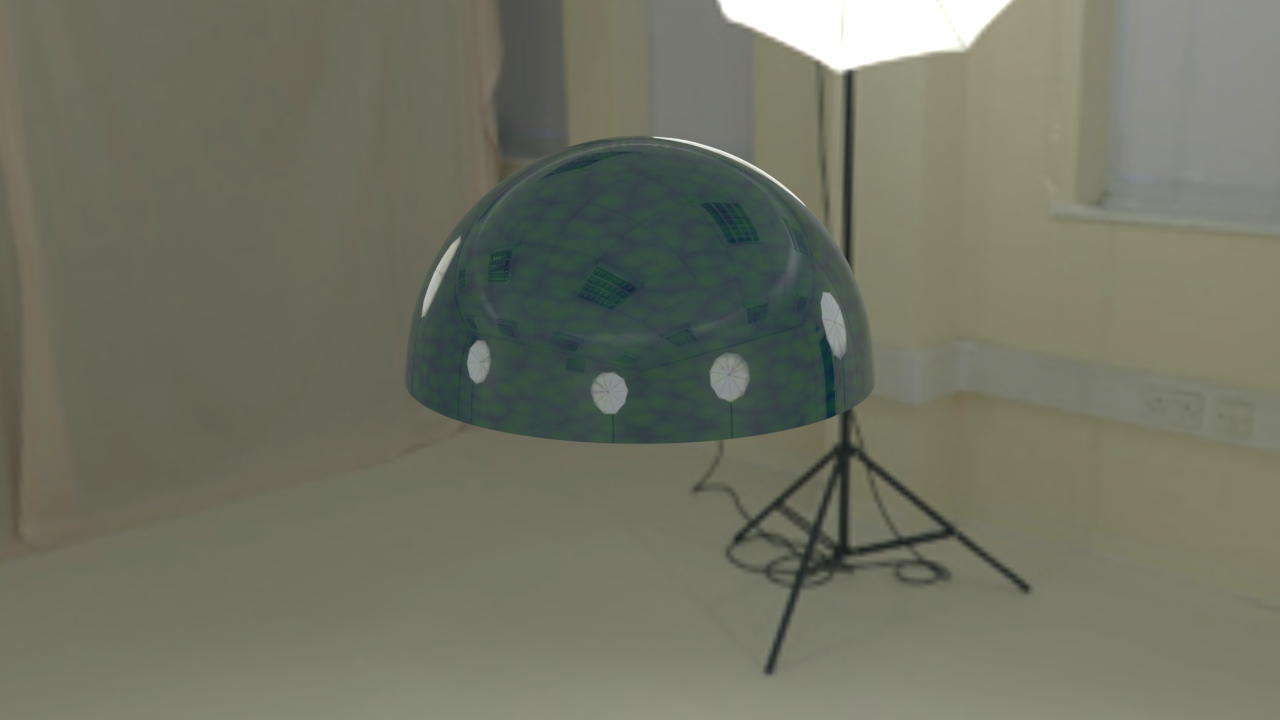
\includegraphics[width=0.33\textwidth]{mapping/mvs_alb_spec/alb_spec_0202}&
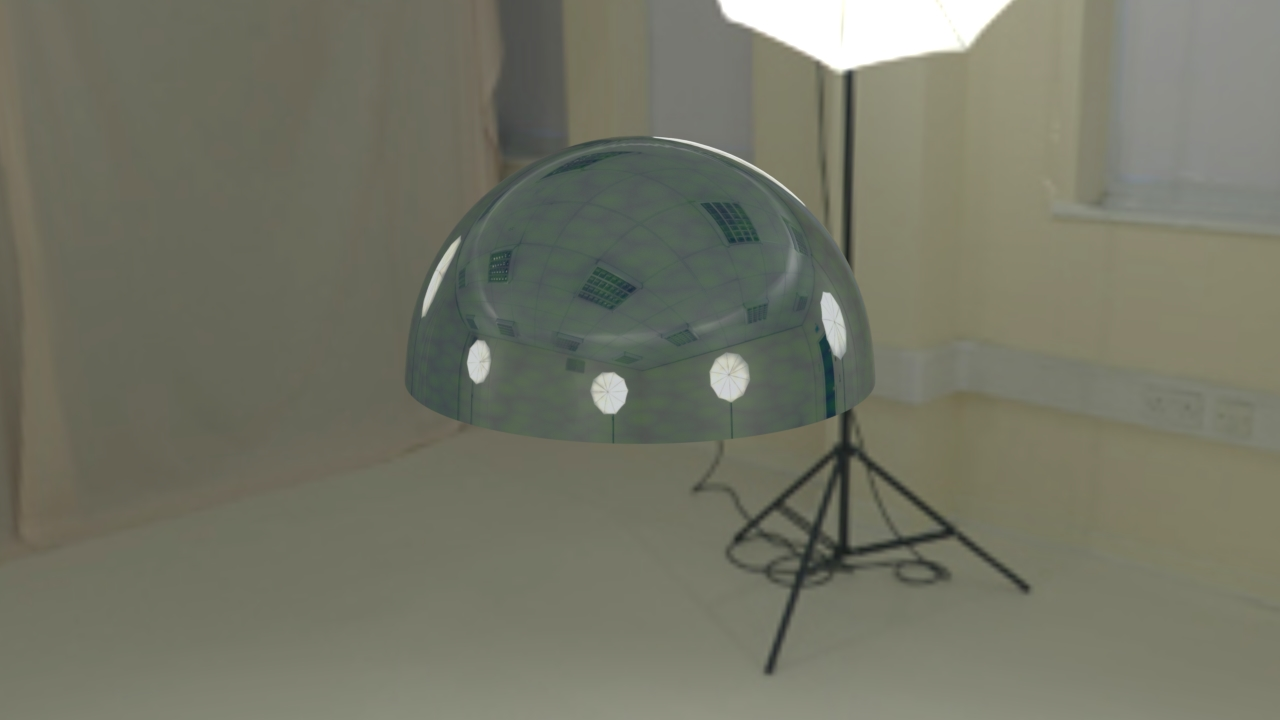
\includegraphics[width=0.33\textwidth]{mapping/mvs_alb_spec/alb_spec_0205}&
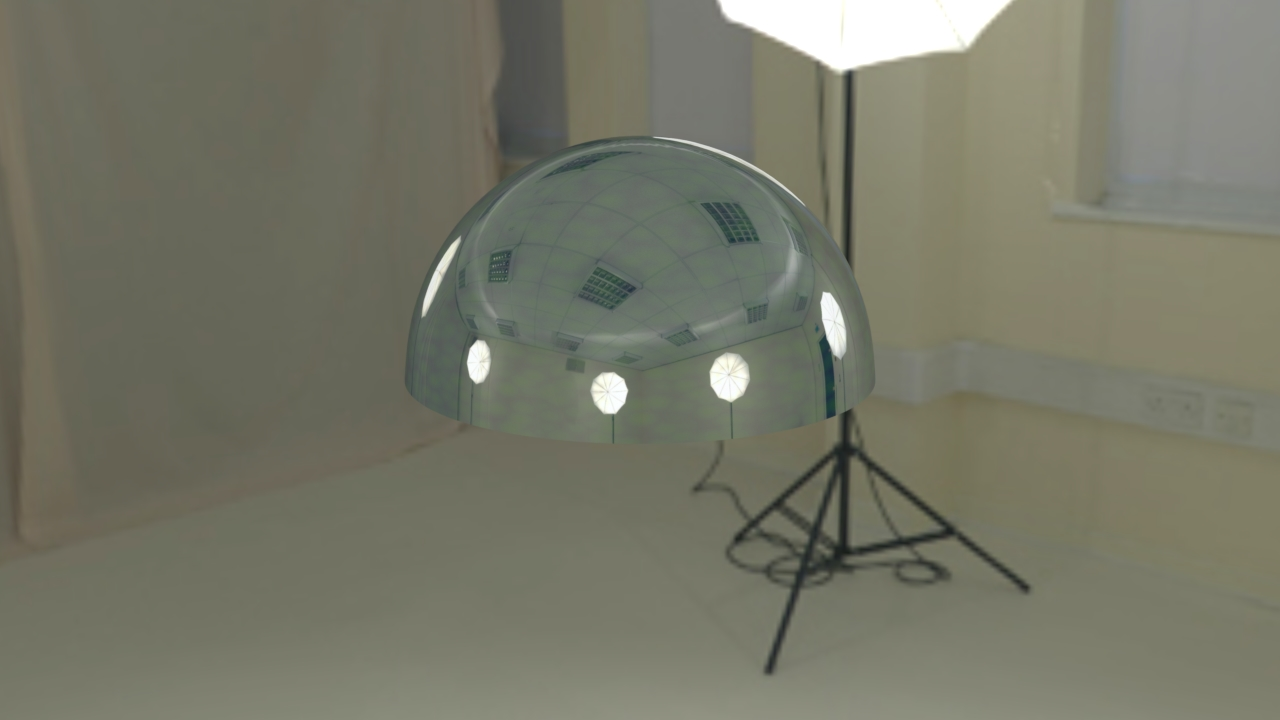
\includegraphics[width=0.33\textwidth]{mapping/mvs_alb_spec/alb_spec_0208}\\
(a) spec: 0.2 & (b) spec: 0.5 & (c) spec: 0.8\\
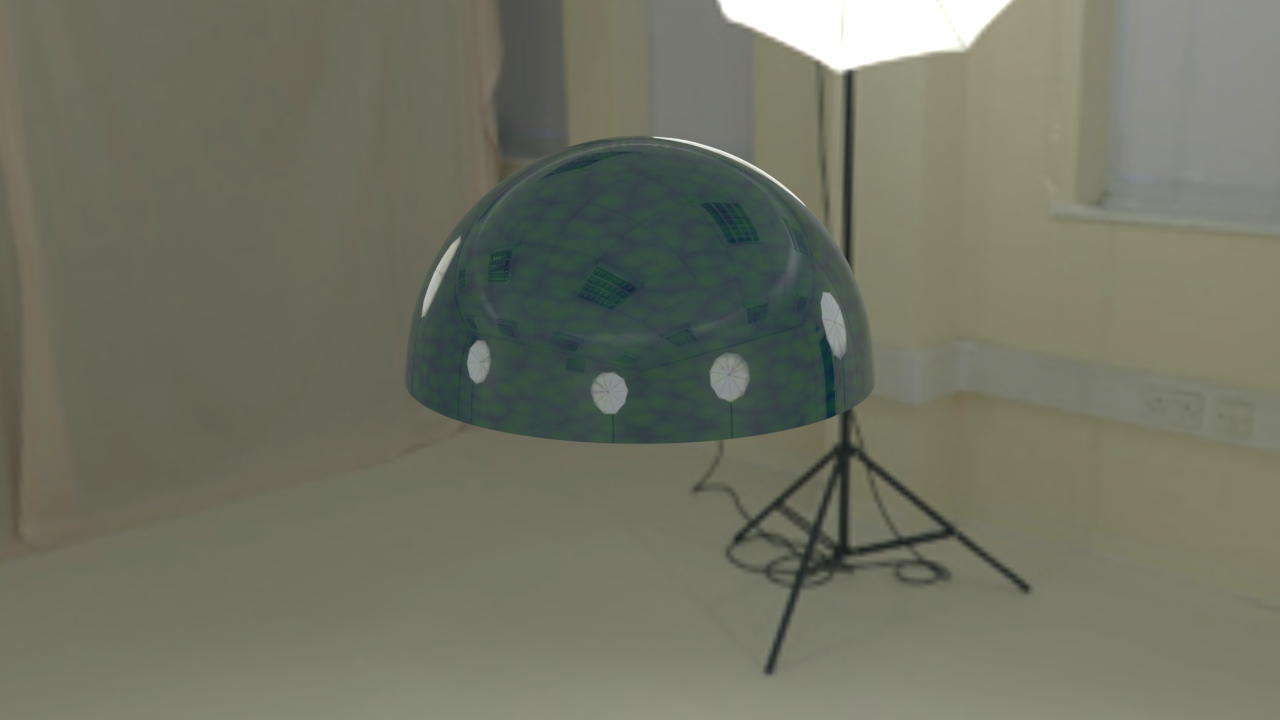
\includegraphics[width=0.33\textwidth]{mapping/mvs_alb_spec/alb_spec_0202}&
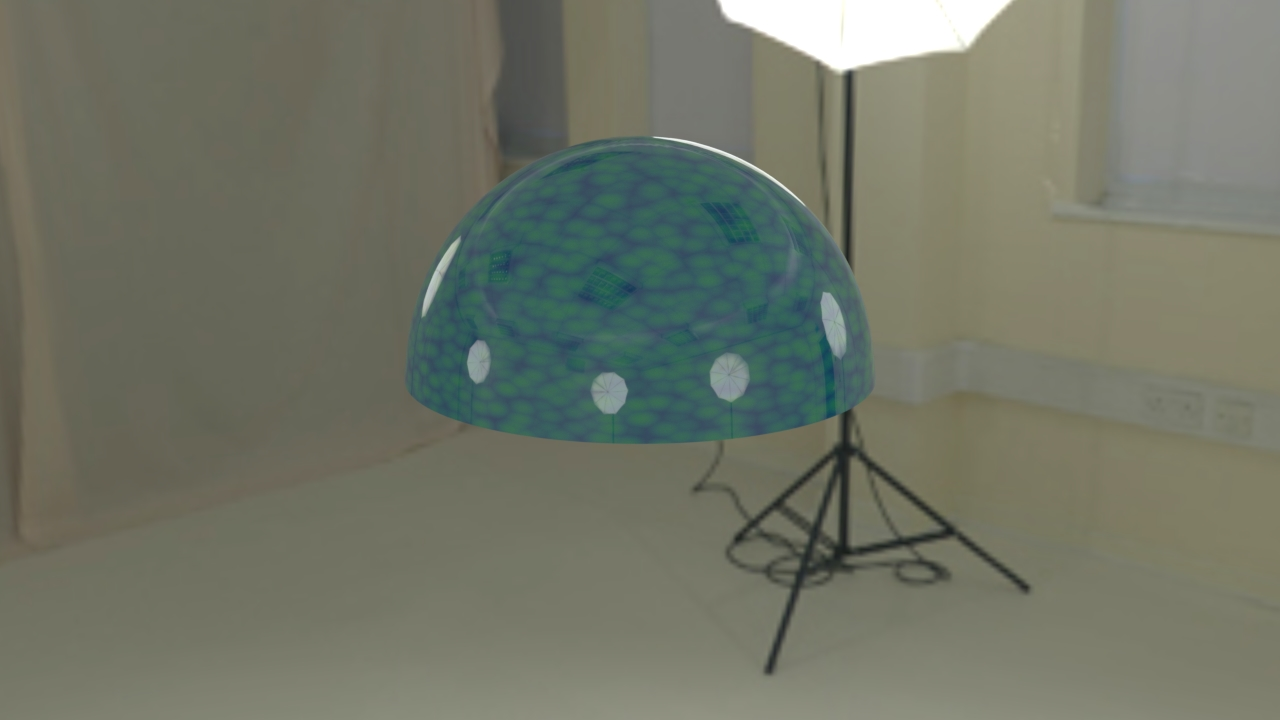
\includegraphics[width=0.33\textwidth]{mapping/mvs_alb_spec/alb_spec_0502}&
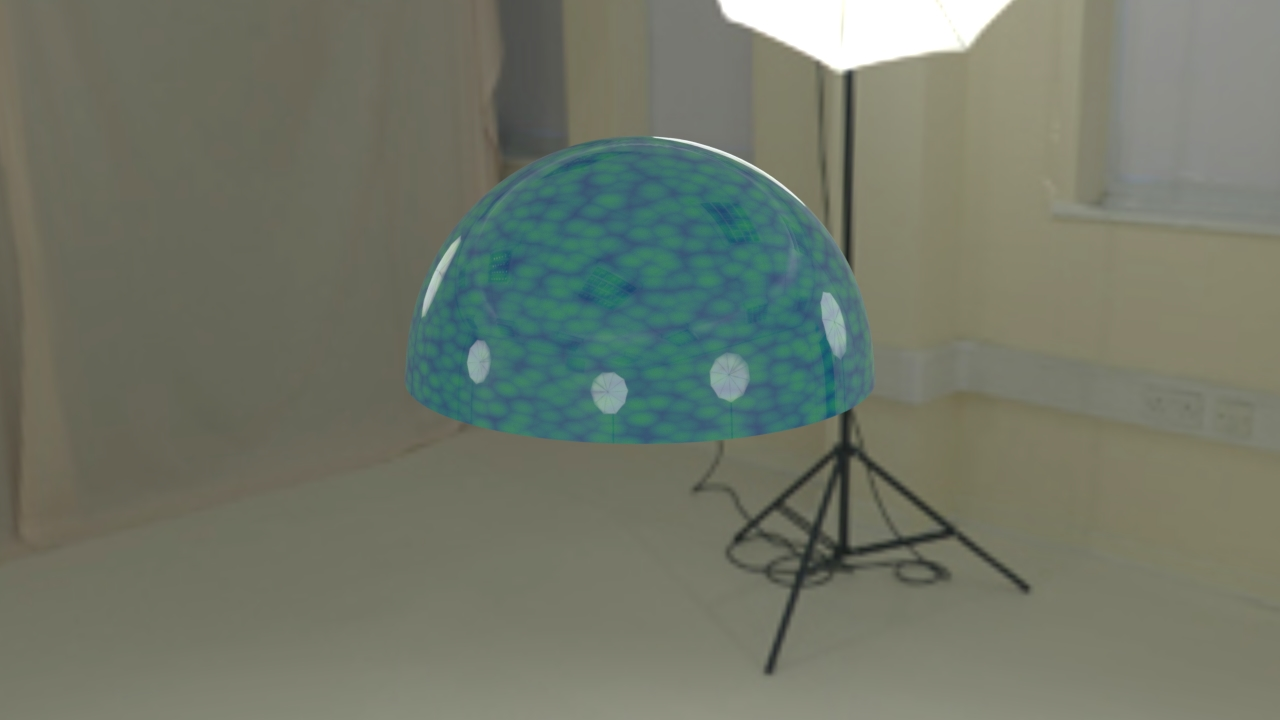
\includegraphics[width=0.33\textwidth]{mapping/mvs_alb_spec/alb_spec_0802}\\
(d) alb: 0.2 & (e) alb: 0.5 & (f) alb: 0.8\\
\end{tabular}
\caption{(a)-(c). The albedo is set as 0.2, (d)-(f). The specularity is set as 0.2. According to energy conservation, as the specular component increases, the diffuse component decreases.}
\label{fig:mvs_alb_spec}
\end{figure}

\textbf{(e) Albedo and Roughness}
albedo and roughness have a negligible effect on the results.

\textbf{(f) Specular and Roughness} 
surface roughness can effectively diminish the specular component and make the surface appear more diffuse. Thus, in theory, roughness should have a positive impact on the reconstruction. However, since specularity is only effective on surface with medium level texture, see Figure~\ref{fig:mvs_depend_check} (b), then roughness is only effective in this case as well. Further, since higher specular, high roughness surfaces visually resemble lower specular surfaces, and achieve similar reconstruction results as well, it makes sense to incorporate the effect of roughness to specularity, and omit roughness for simplicity.

\subsubsection{Effective Properties: PMVS} 
The effective properties of PMVS are: texture, albedo, and specular, as shown in Table~\ref{tab:mvs_depend_prop}. Interestingly, we discovered that specularity has a more substantially negative impact on less textured, lower albedo surfaces. For instance, high specularity does not have a severely negative impact on highly textured surfaces.
\begin{table}[!htbp]
  \centering
  \begin{tabular}{l*{4}{c}}
  \hline
  \textbf{Metric} & Texture & Albedo & Specular & Roughness\\
  \hline
  Accuracy & \checkmark & \checkmark & \checkmark & \ding{55}\\
  Completeness & \checkmark & \checkmark & \checkmark & \ding{55}\\
  \hline
  \end{tabular}
  \caption{The \textit{effective problem domain} of PMVS in terms of accuracy and completeness.}
  \label{tab:mvs_depend_prop}
\end{table}

\subsection{EPD: EPS}
\label{sec:ps_epd}
We investigate the impact of each property on the performance of example-based PS in terms of angular error under varied combinations of properties. The settings of the properties are listed in Table~\ref{tab:pairwise_prob_cond}.

\begin{sidewaysfigure}[!htbp]
\begin{tabular}{ccc}
\includegraphics[width=0.3\textwidth]{mapping/depend_check/ps_tex_alb}&
\includegraphics[width=0.3\textwidth]{mapping/depend_check/ps_tex_spec}&
\includegraphics[width=0.3\textwidth]{mapping/depend_check/ps_tex_rough}\\
(a) & (b) &(c)\\
\includegraphics[width=0.3\textwidth]{mapping/depend_check/ps_alb_spec}&
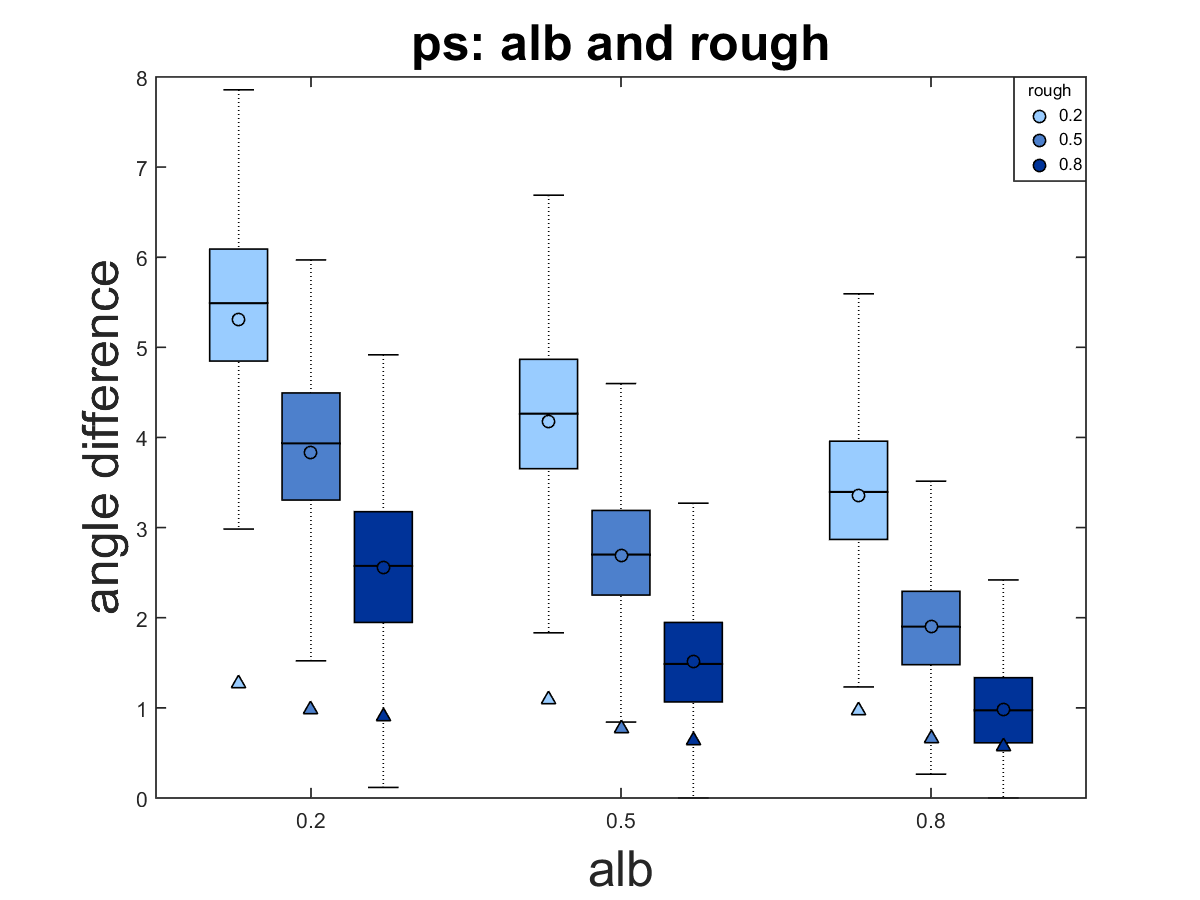
\includegraphics[width=0.3\textwidth]{mapping/depend_check/ps_alb_rough}&
\includegraphics[width=0.3\textwidth]{mapping/depend_check/ps_spec_rough}\\
(d) & (e) & (f)\\
\end{tabular}
\caption{Performance of Example-based PS under six pairwise conditions. For instance, (a) shows the performance under changing \textit{texture} and \textit{albedo} values. The property values are assigned based on the settings in Table~\ref{tab:ps_depend_check_params} (a).}
\label{fig:ps_depend_check}
\end{sidewaysfigure}

\textbf{(a) Texture and Albedo} 
texture has no significant effect while albedo has a positive effect on normal estimation.

\textbf{(b) Texture and Specularity} 
texture has no effect while specularity has a negative effect on normal estimation, which is manifested by the increased interquartile range and skewness. The explaination is as follows: normals in the specular regions are poorly estimated while the rest of the surface is reliably estimated, as shown in Figure~\ref{fig:ps_tex_spec}. This explains the increased mean and interquartile values as shown in Figure~\ref{fig:ps_depend_check} (b).
\begin{figure}[!htbp]
\centering
\begin{tabular}{c|ccc}
Image & Normal map & Height map & Angular error\\
\hline\\
\includegraphics[width=0.33\textwidth]{mapping/ps_tex_spec/0502_0001}&
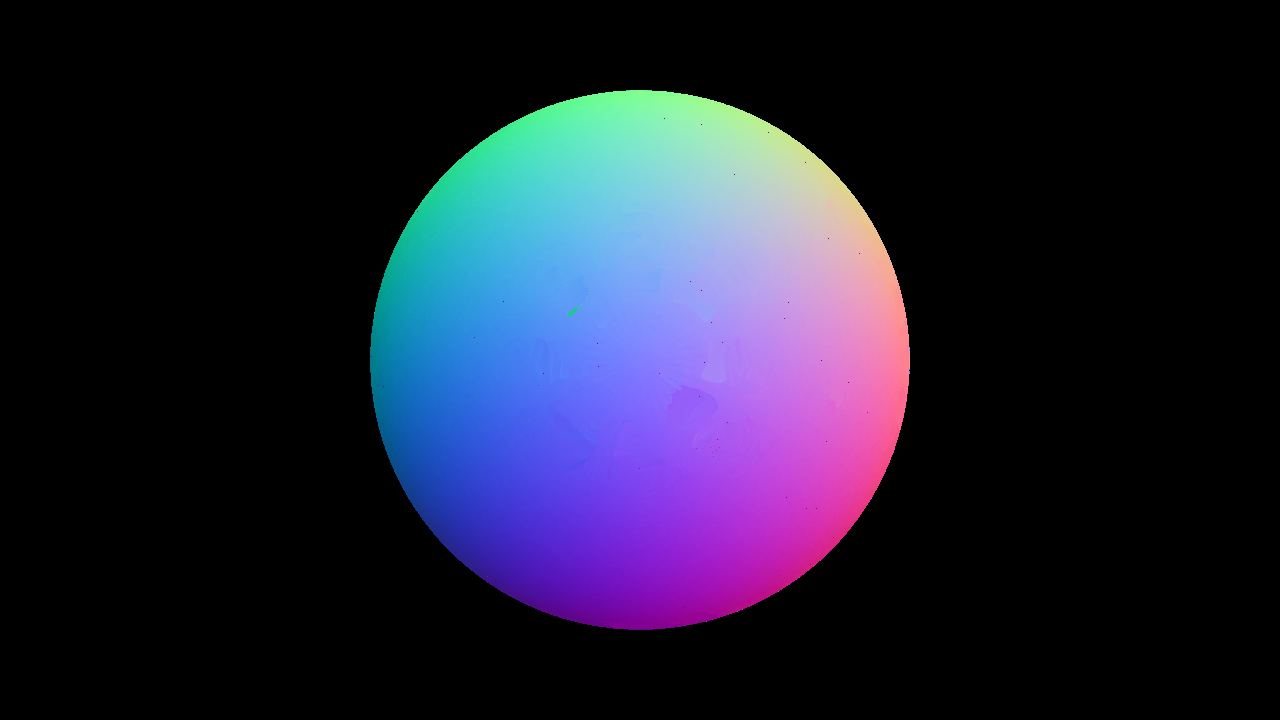
\includegraphics[width=0.33\textwidth]{mapping/ps_tex_spec/0502_normal}&
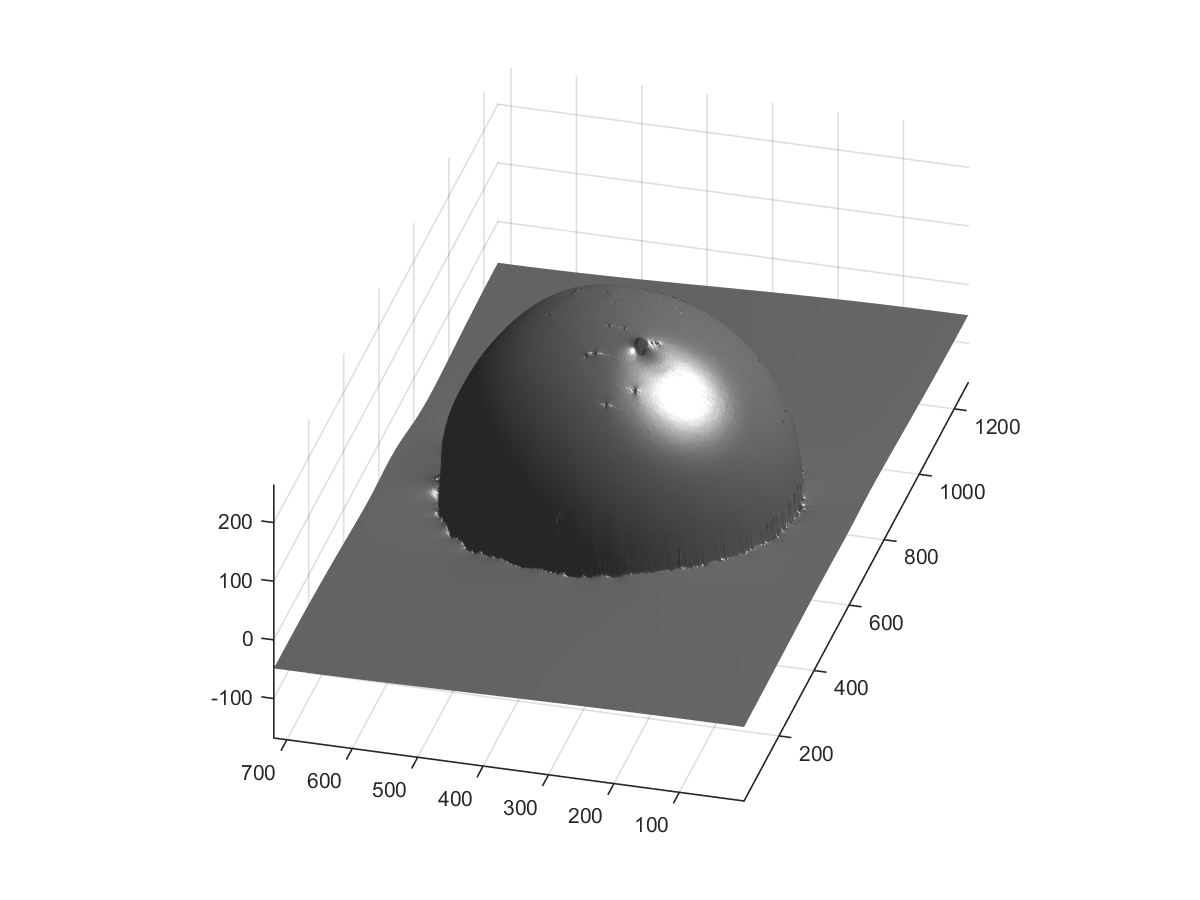
\includegraphics[width=0.25\textwidth]{mapping/ps_tex_spec/0502_dmap}&
\includegraphics[width=0.06\textwidth]{mapping/ps_tex_spec/0502_ang_error}\\
 & spec: 0.2 & \\
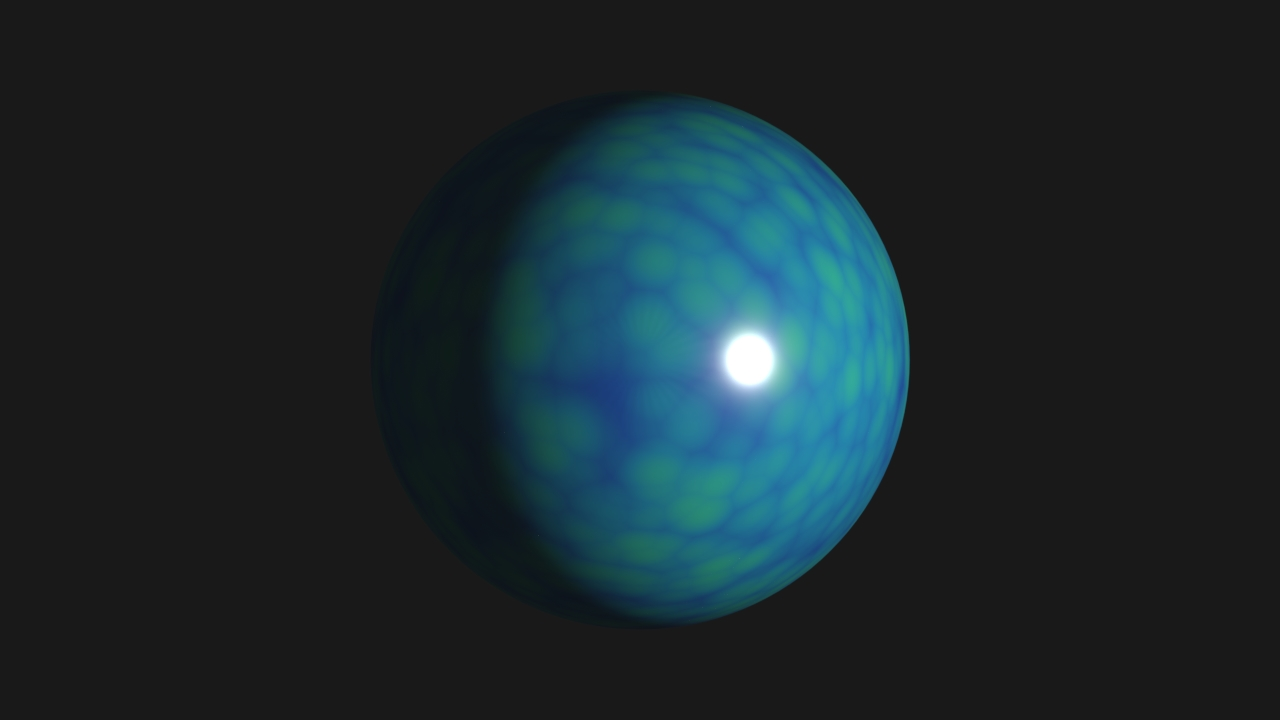
\includegraphics[width=0.33\textwidth]{mapping/ps_tex_spec/0505_0001}&
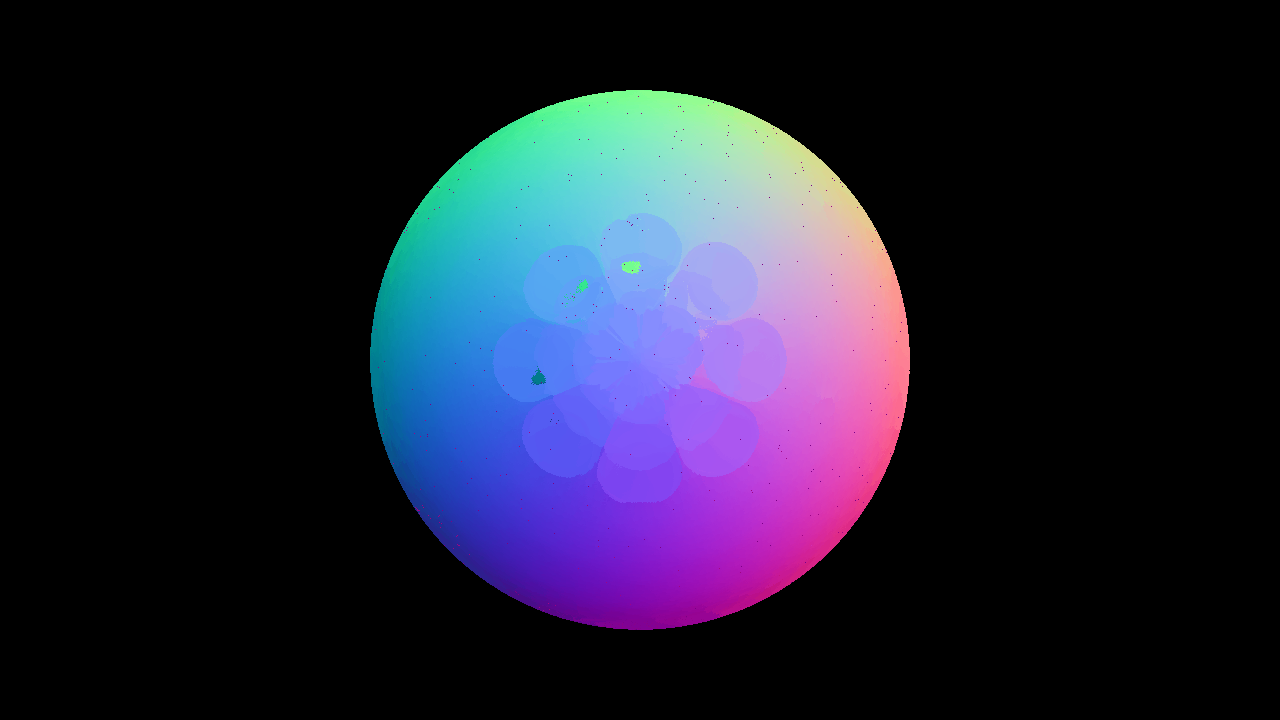
\includegraphics[width=0.33\textwidth]{mapping/ps_tex_spec/0505_normal}&
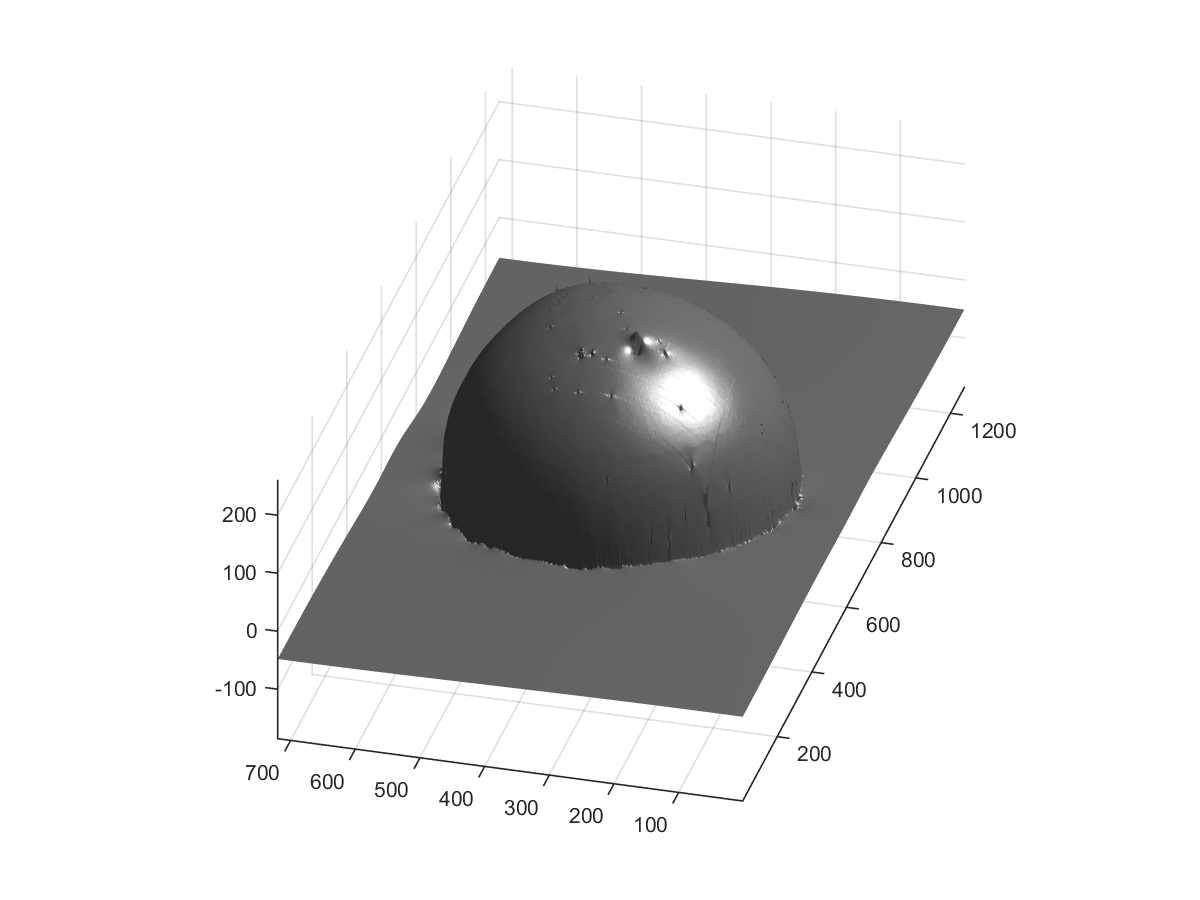
\includegraphics[width=0.25\textwidth]{mapping/ps_tex_spec/0505_dmap}&
\includegraphics[width=0.06\textwidth]{mapping/ps_tex_spec/0505_ang_error}\\
 & spec: 0.5 & \\
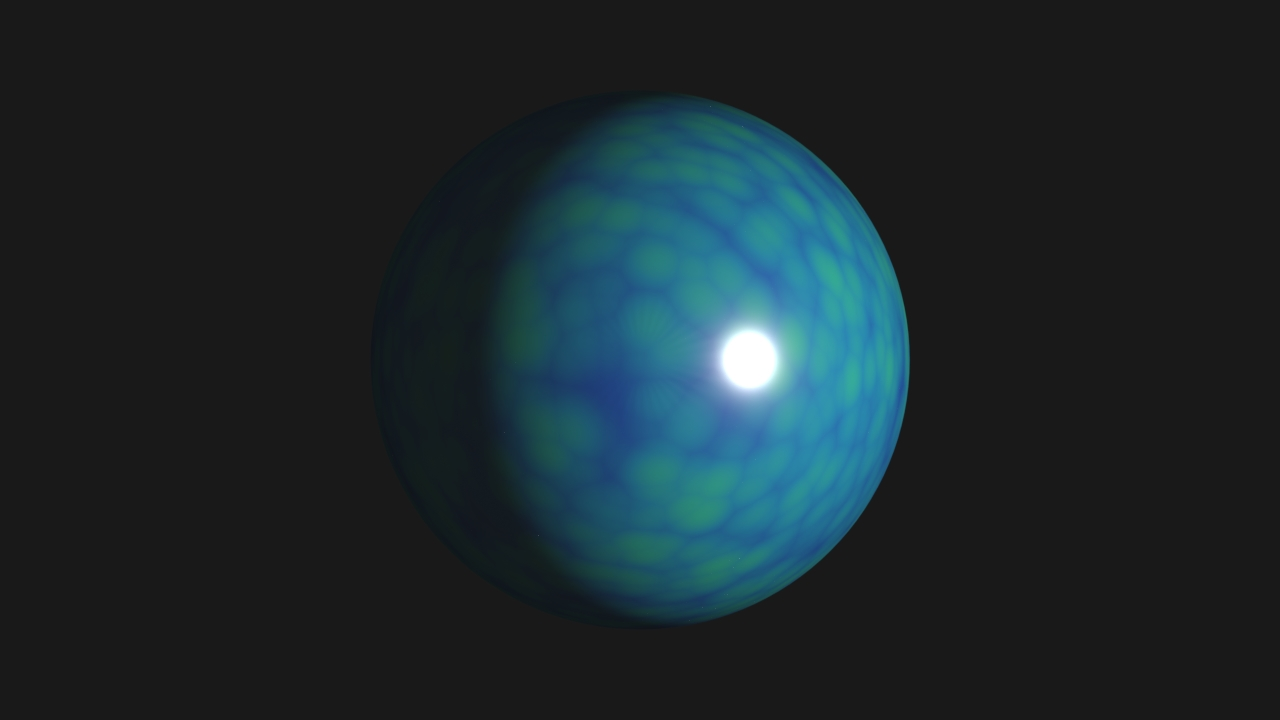
\includegraphics[width=0.33\textwidth]{mapping/ps_tex_spec/0508_0001}&
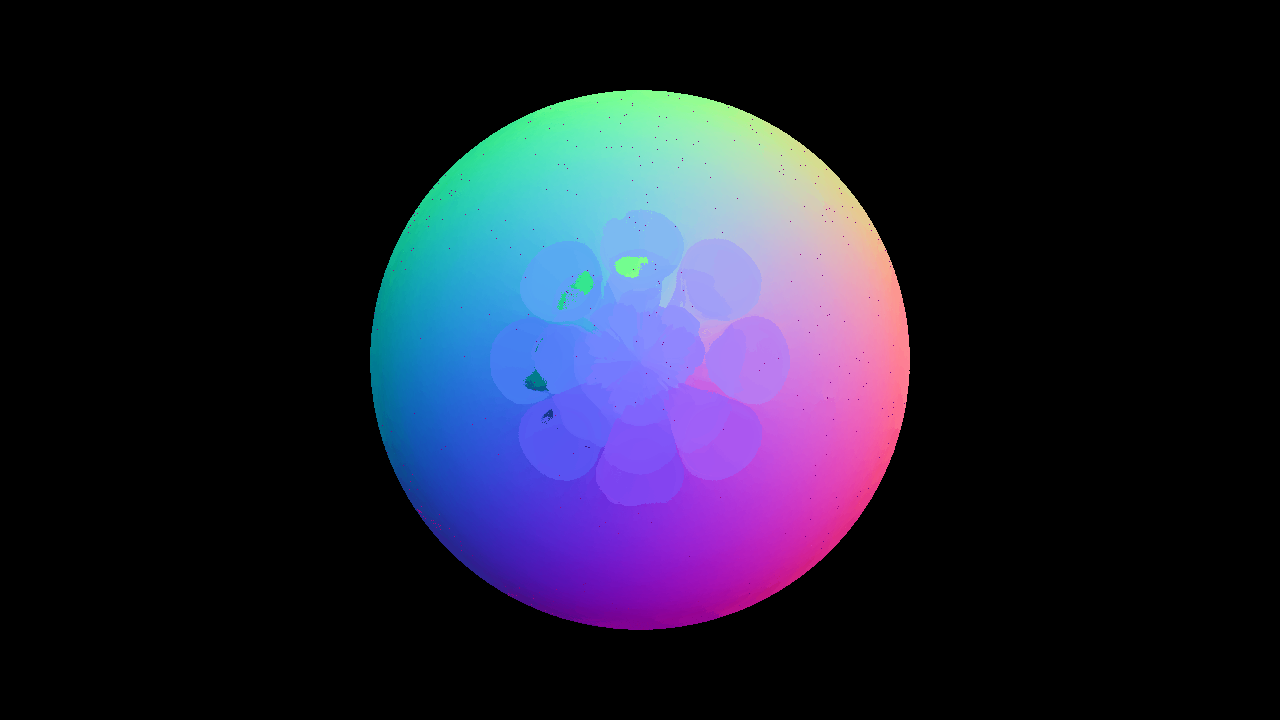
\includegraphics[width=0.33\textwidth]{mapping/ps_tex_spec/0508_normal}&
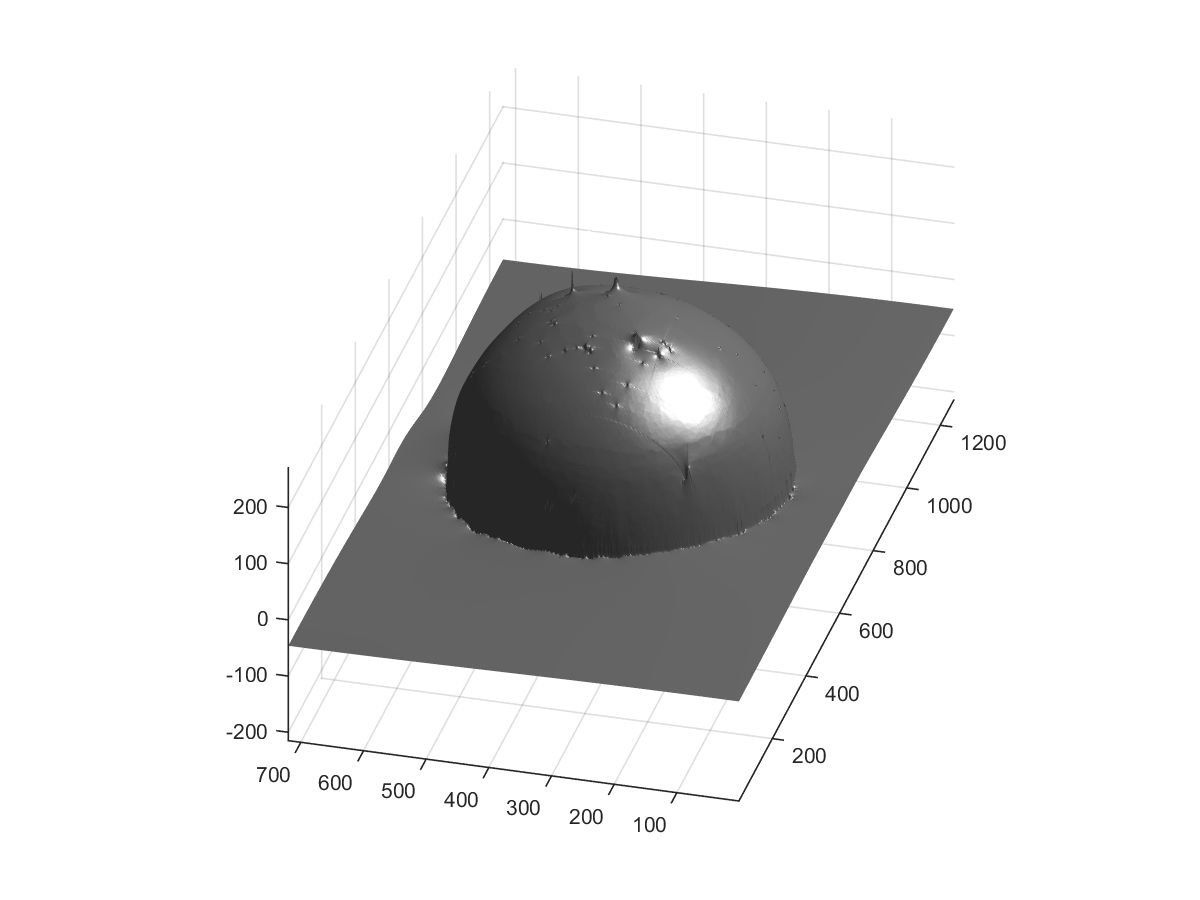
\includegraphics[width=0.25\textwidth]{mapping/ps_tex_spec/0508_dmap}&
\includegraphics[width=0.06\textwidth]{mapping/ps_tex_spec/0508_ang_error}\\
 & spec: 0.8 & \\
\end{tabular}
\caption{(a)-(c). The texture is set as 0.5. The estimated normal map and recovered surface becomes consistently worse as the specular level rises, which is consistent with the quantitative results from Figure~\ref{fig:ps_depend_check} (b).}
\label{fig:ps_tex_spec}
\end{figure}

\textbf{(c) Texture and Roughness} 
texture has no effect while roughness has a positive effect on normal estimation.

\textbf{(d) Albedo and Specular} 
the albedo has a positive impact on normal estimation (see Figure~\ref{fig:ps_alb_spec} (a)-(c)), whereas the specularity has a negative impact on normal estimation (see Figure~\ref{fig:ps_alb_spec} (d)-(f)).
\begin{figure}[!htbp]
\centering
\begin{tabular}{c|ccc}
Image & Normal map & Height map & Angular error\\
\hline\\
% 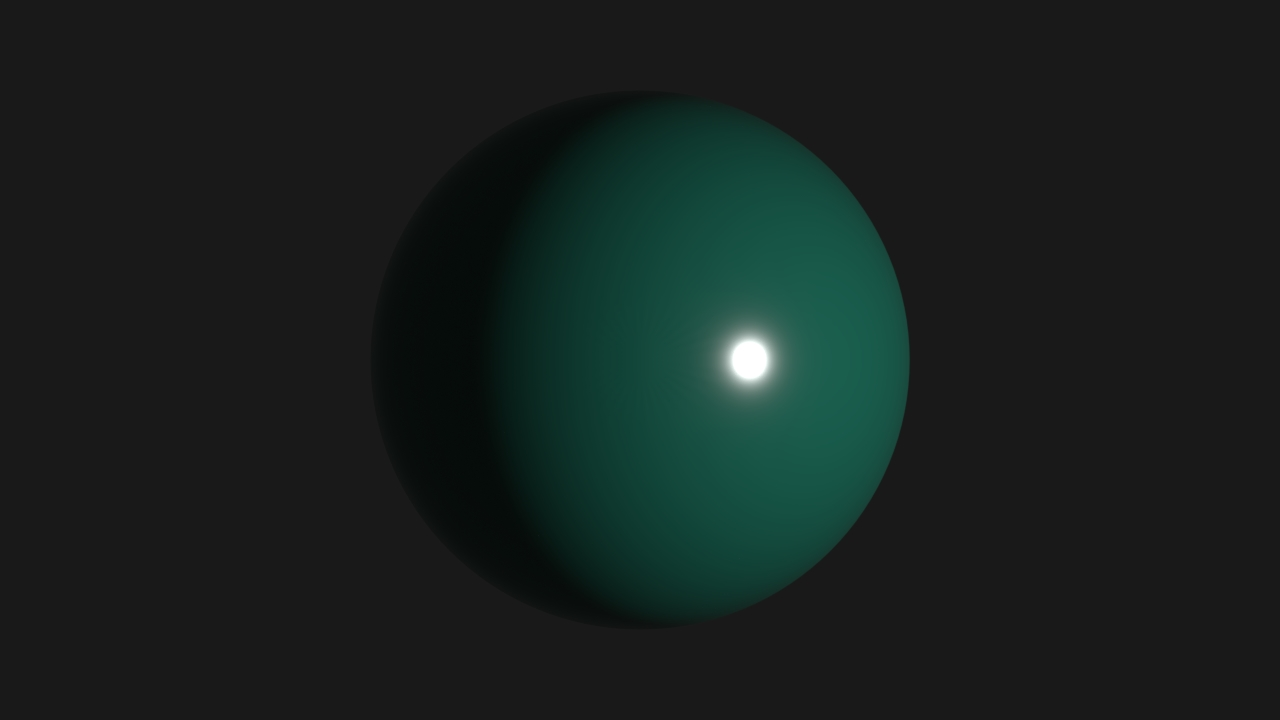
\includegraphics[width=0.33\textwidth]{mapping/ps_alb_spec/0202_0001}&
% 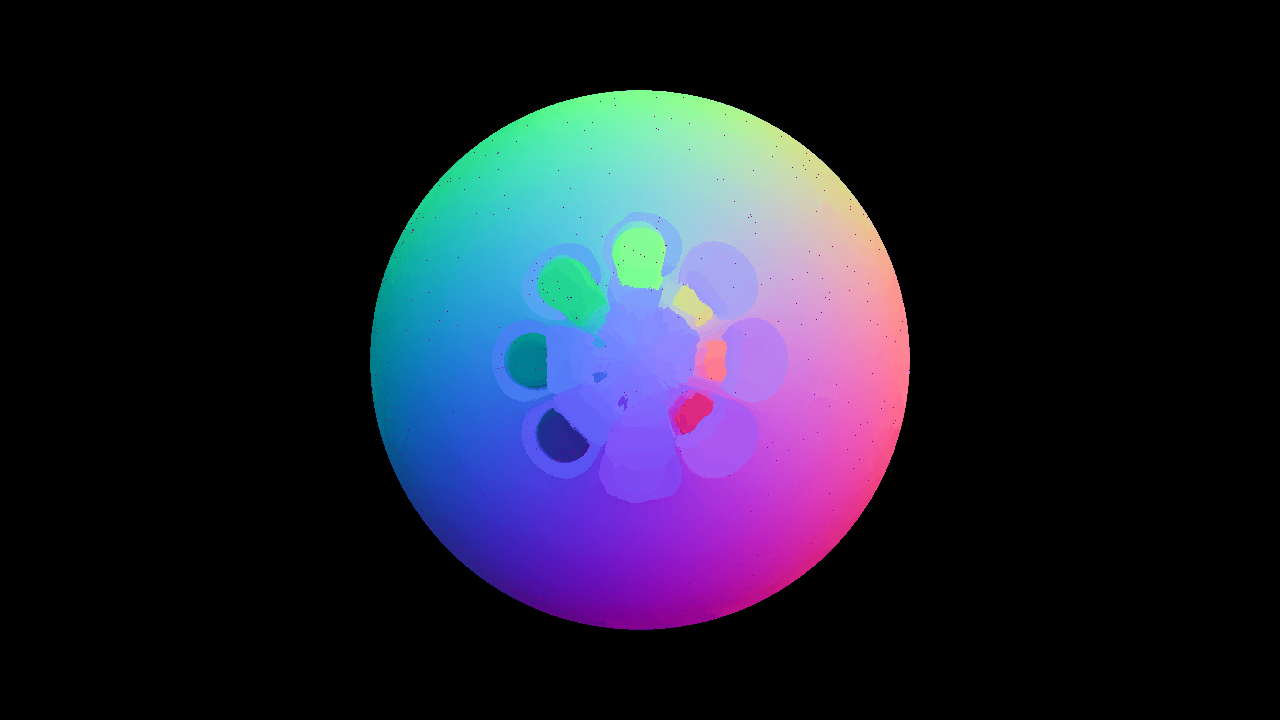
\includegraphics[width=0.33\textwidth]{mapping/ps_alb_spec/0202_normal}&
% 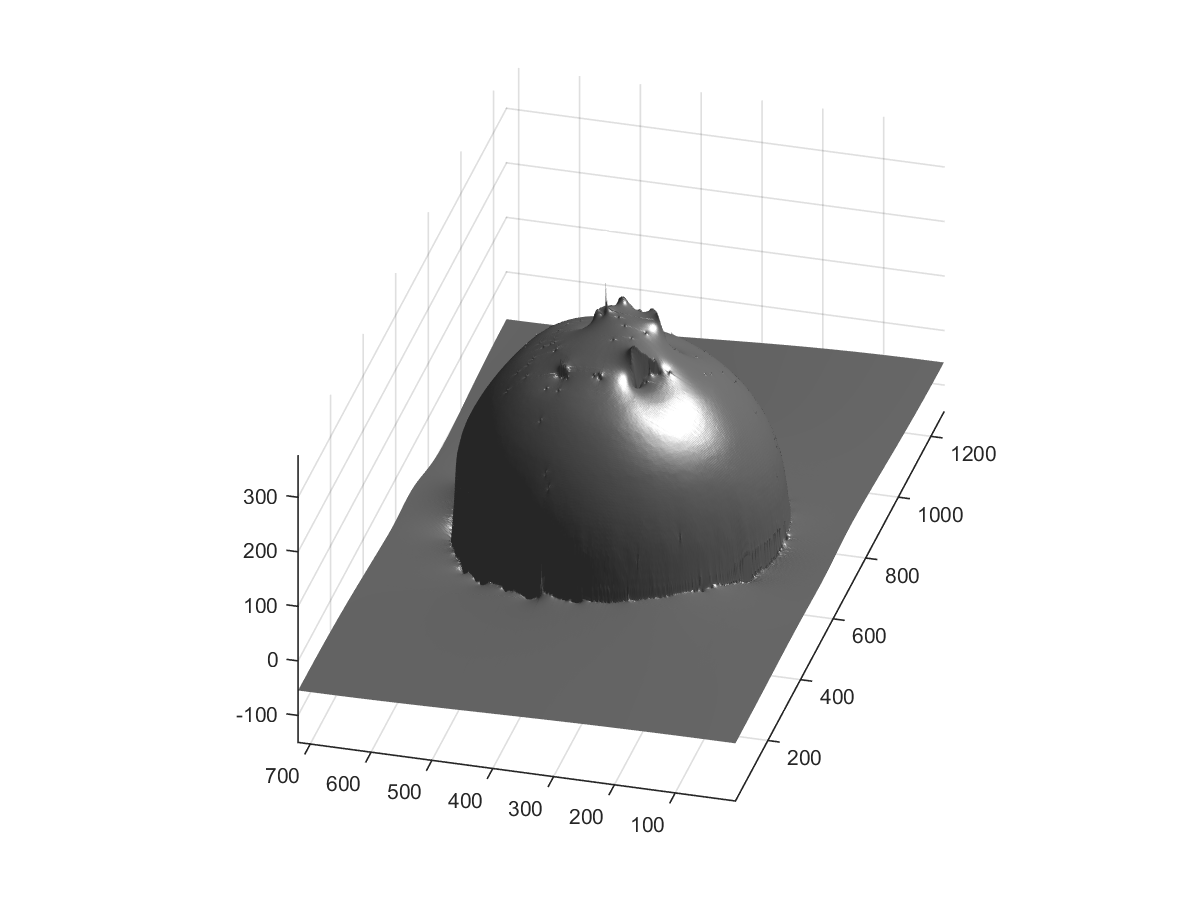
\includegraphics[width=0.25\textwidth]{mapping/ps_alb_spec/0202_dmap}&
% \includegraphics[width=0.06\textwidth]{mapping/ps_alb_spec/0202_ang_error}\\
%  & (a) albedo: 0.2, spec: 0.2 & \\
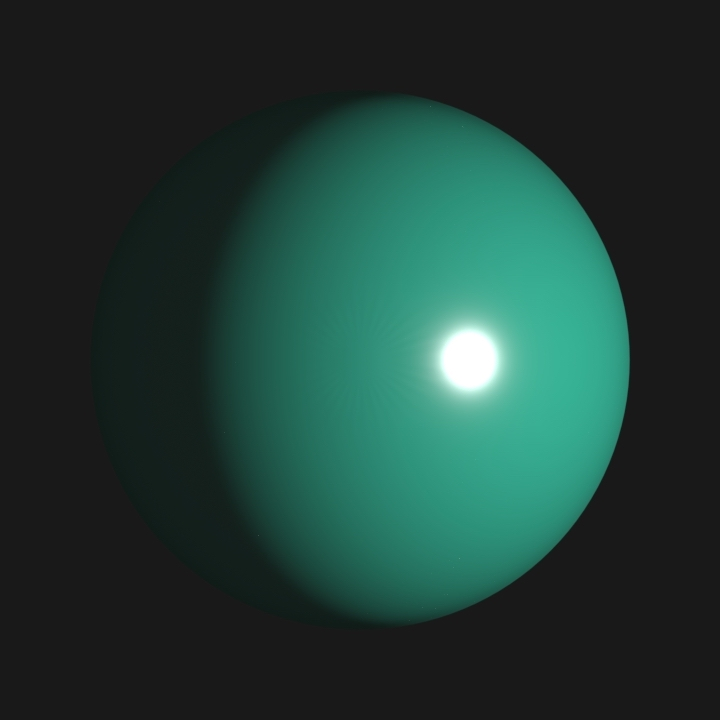
\includegraphics[width=0.33\textwidth]{mapping/ps_alb_spec/0802_0001}&
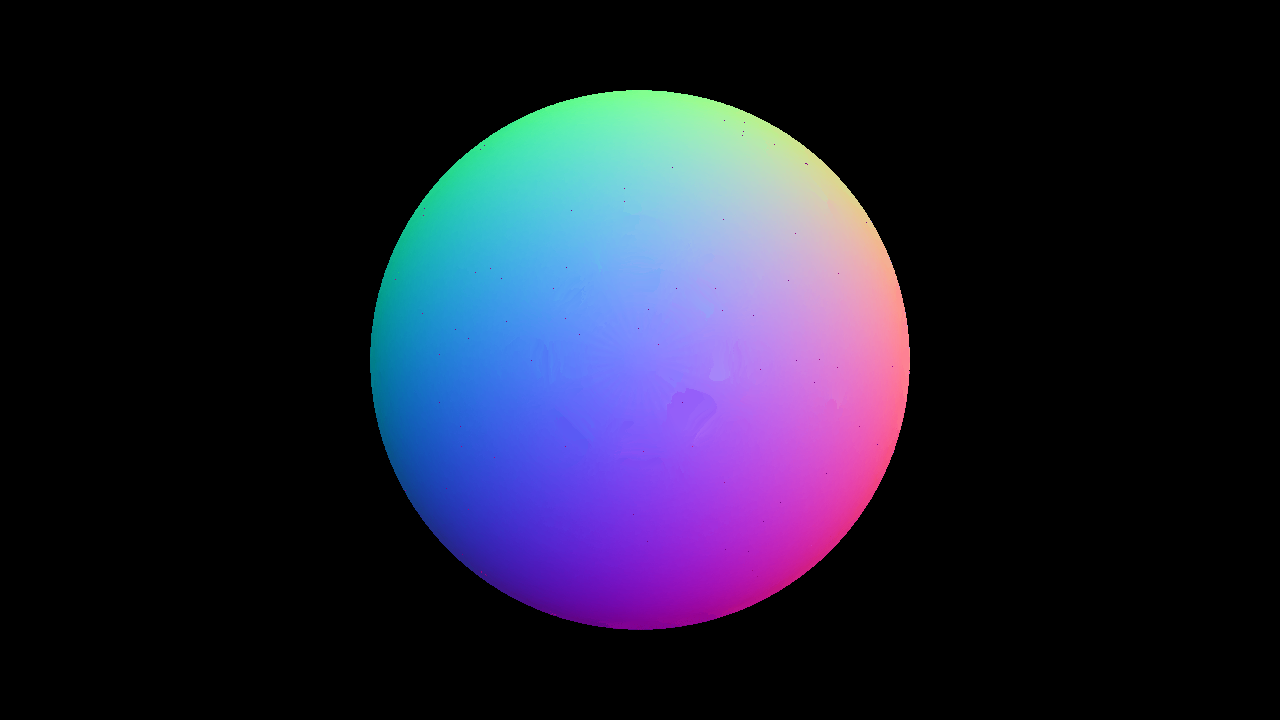
\includegraphics[width=0.33\textwidth]{mapping/ps_alb_spec/0802_normal}&
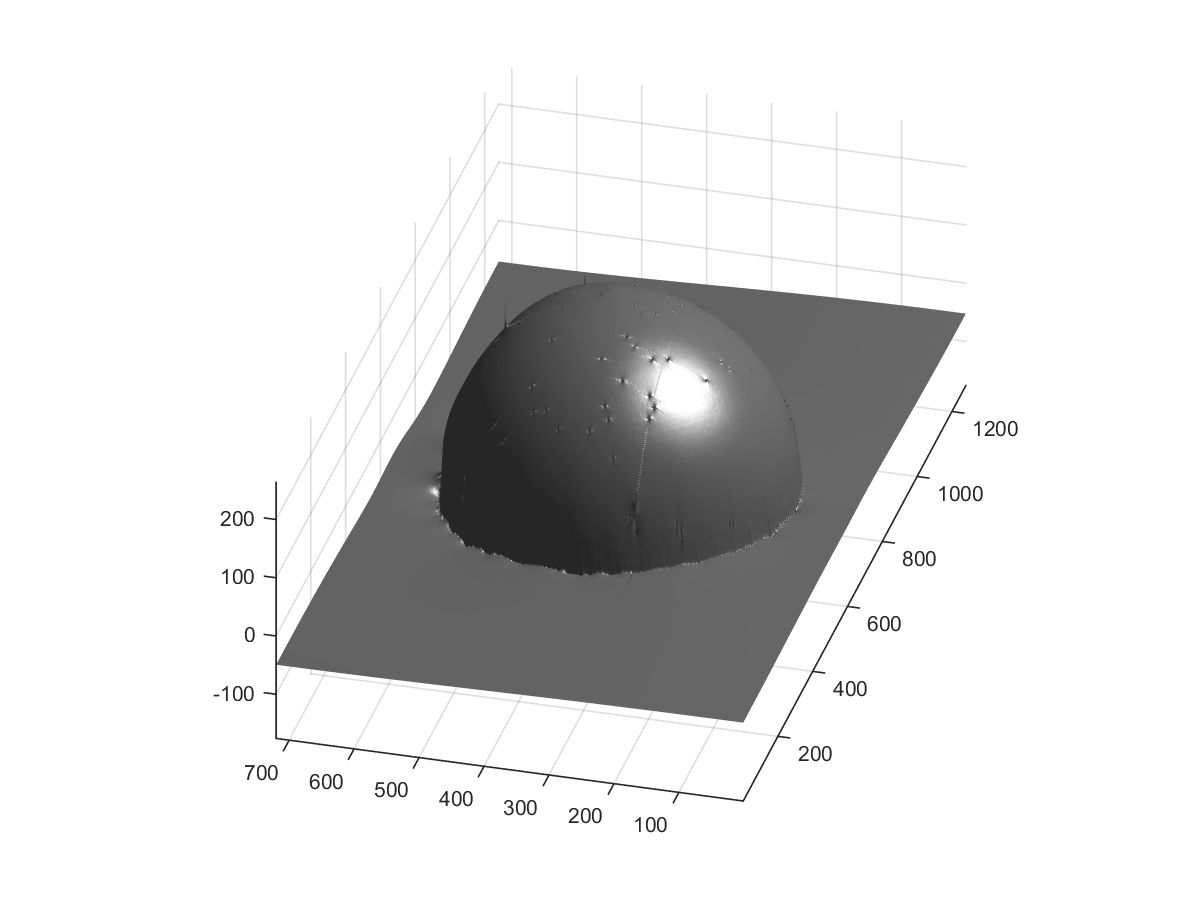
\includegraphics[width=0.25\textwidth]{mapping/ps_alb_spec/0802_dmap}&
\includegraphics[width=0.06\textwidth]{mapping/ps_alb_spec/0802_ang_error}\\
 & (a) albedo: 0.8, spec: 0.2 & \\
\includegraphics[width=0.33\textwidth]{mapping/ps_alb_spec/0502_0001}&
\includegraphics[width=0.33\textwidth]{mapping/ps_alb_spec/0502_normal}&
\includegraphics[width=0.25\textwidth]{mapping/ps_alb_spec/0502_dmap}&
\includegraphics[width=0.06\textwidth]{mapping/ps_alb_spec/0502_ang_error}\\
 & (b) albedo: 0.5, spec: 0.2 & \\
\includegraphics[width=0.33\textwidth]{mapping/ps_alb_spec/0202_0001}&
\includegraphics[width=0.33\textwidth]{mapping/ps_alb_spec/0202_normal}&
\includegraphics[width=0.25\textwidth]{mapping/ps_alb_spec/0202_dmap}&
\includegraphics[width=0.06\textwidth]{mapping/ps_alb_spec/0202_ang_error}\\
 & (c) albedo: 0.2, spec: 0.2 & \\
\includegraphics[width=0.33\textwidth]{mapping/ps_alb_spec/0205_0001}&
\includegraphics[width=0.33\textwidth]{mapping/ps_alb_spec/0205_normal}&
\includegraphics[width=0.25\textwidth]{mapping/ps_alb_spec/0205_dmap}&
\includegraphics[width=0.06\textwidth]{mapping/ps_alb_spec/0205_ang_error}\\
 & (d) albedo: 0.2, spec: 0.5 & \\
\includegraphics[width=0.33\textwidth]{mapping/ps_alb_spec/0208_0001}&
\includegraphics[width=0.33\textwidth]{mapping/ps_alb_spec/0208_normal}&
\includegraphics[width=0.25\textwidth]{mapping/ps_alb_spec/0208_dmap}&
\includegraphics[width=0.06\textwidth]{mapping/ps_alb_spec/0208_ang_error}\\
 & (e) albedo: 0.2, spec: 0.8 & \\
\end{tabular}
\caption{According to energy conservation, as the specular component increases, the diffuse component decreases. (a)-(c): the estimated normal map and recovered height map become consistently worse as the albedo decreases; (c)-(e): the estimated normal map and recovered height map become consistently worse as the specularity increases.}
\label{fig:ps_alb_spec}
\end{figure}

\textbf{(e) Albedo and Roughness} 
both albedo and roughness have a positive effect on normal estimation.

\textbf{(f) Specular and Roughness} 
specularity has a negative impact on normal estimation, while the effect of roughness is more complicated. We observed that the reconstruction becomes worse for medium roughness, which is counter-intuitive at first sight. However, we argue that it's because the roughness is not strong enough to counteract the specular component, causing a smoothed and blurred specular region with larger area, thus leading to a poorer normal estimation. See Figure~\ref{fig:ps_spec_rough} for visual examples.
\begin{figure}[!htbp]
\centering
\begin{tabular}{c|ccc}
  Image & Normal map & Height map & Angular error\\
  \hline\\
  \includegraphics[width=0.33\textwidth]{mapping/ps_spec_rough/0802_0001}&
  \includegraphics[width=0.33\textwidth]{mapping/ps_spec_rough/0802_normal}&
  \includegraphics[width=0.25\textwidth]{mapping/ps_spec_rough/0802_dmap}&
  \includegraphics[width=0.06\textwidth]{mapping/ps_spec_rough/0802_ang_error}\\
  & (a). rough: 0.2\\
  \includegraphics[width=0.33\textwidth]{mapping/ps_spec_rough/0805_0001}&
  \includegraphics[width=0.33\textwidth]{mapping/ps_spec_rough/0805_normal}&
  \includegraphics[width=0.25\textwidth]{mapping/ps_spec_rough/0805_dmap}&
  \includegraphics[width=0.06\textwidth]{mapping/ps_spec_rough/0805_ang_error}\\
  & (b). rough: 0.5\\
  \includegraphics[width=0.33\textwidth]{mapping/ps_spec_rough/0808_0001}&
  \includegraphics[width=0.33\textwidth]{mapping/ps_spec_rough/0808_normal}&
  \includegraphics[width=0.25\textwidth]{mapping/ps_spec_rough/0808_dmap}&
  \includegraphics[width=0.06\textwidth]{mapping/ps_spec_rough/0808_ang_error}\\
  & (c). rough: 0.8\\
\end{tabular}
\caption{The effect of roughness on PS. Albedo is set as 0.8, and specular is set as 0.8. (b) demonstrates that a medium level roughness would lead to worse normal estimation since it blurs the specular lobe.}
\label{fig:ps_spec_rough}
\end{figure}

\subsubsection{Effective Properties: EPS} 
The properties that have an impact on EPS are: albedo, specularity, and roughness, as shown in Table~\ref{tab:ps_depend_prop}. Interestingly, we have discovered that medium level roughness can have a negative impact on normal estimation by blur the specular lobe, as shown in Figure~\ref{fig:ps_spec_rough}.
\begin{table}[!htbp]
  \centering
  \begin{tabular}{l*{5}{c}}
  \hline
  \textbf{Metric} & Texture & Albedo & Specular & Roughness\\
  \hline
  Angle difference & \ding{55} & \checkmark & \checkmark & \checkmark\\
  \hline
  \end{tabular}
  \caption{The \textit{effective problem domain} of EPS in terms of the \textit{angular error}.}
  \label{tab:ps_depend_prop}
\end{table}

\subsection{EPD: GSL}
\label{sec:sl_epd}
We investigate the impact of each property on the performance of Gray-code SL in terms of accuracy and completeness under a varied combination of properties. The settings of properties are listed in Table~\ref{tab:pairwise_prob_cond}.

\begin{sidewaysfigure}[!htbp]
\begin{tabular}{ccc}
\includegraphics[width=0.3\textwidth]{mapping/depend_check/sl_tex_alb}&
\includegraphics[width=0.3\textwidth]{mapping/depend_check/sl_tex_spec}&
\includegraphics[width=0.3\textwidth]{mapping/depend_check/sl_tex_rough}\\
(a) & (b) & (c)\\
\includegraphics[width=0.3\textwidth]{mapping/depend_check/sl_alb_spec}&
\includegraphics[width=0.3\textwidth]{mapping/depend_check/sl_alb_rough}&
\includegraphics[width=0.3\textwidth]{mapping/depend_check/sl_spec_rough}\\
(d) & (e) & (f)\\
\end{tabular}
\caption{Performance of Gray-encoded SL under six pairwise conditions. For instance, (a) shows the performance under changing \textit{texture} and \textit{albedo} values. The property values are assigned based on settings in Table~\ref{tab:sl_depend_check_params} (a).}
\label{fig:sl_depend_check}
\end{sidewaysfigure}

\textbf{(a) Texture and Albedo} 
texture has no significant effect, whereas albedo has a positive effect on completeness. Both properties have no significant effect on accuracy.

\textbf{(b) Texture and Specular} 
texture has no significant effect whereas specular has a negative effect on completeness. Both properties have no significant effect on accuracy.

\textbf{(c) Texture and Roughness} 
neither texture nor roughness has a significant effect on accuracy and completeness.

\textbf{(d) Albedo and Specularity} 
albedo has a positive effect (see Figure~\ref{fig:sl_alb_spec} (a)-(c)) whereas specularity has a negative effect on completeness (see Figure~\ref{fig:sl_alb_spec} (d)-(f)). Interestingly, similar to EPS, the positive effect of albedo gets more significant with higher specularity while the negative effect of specularity becomes less substantial as albedo increases (see Figure~\ref{fig:sl_depend_check} (d)). Neither property has a significant effect on accuracy.
\begin{figure}[!htbp]
\centering
\begin{tabular}{ccc}
\includegraphics[width=0.33\textwidth]{mapping/sl_alb_spec/sl_00020202}&
\includegraphics[width=0.33\textwidth]{mapping/sl_alb_spec/sl_00050202}&
\includegraphics[width=0.33\textwidth]{mapping/sl_alb_spec/sl_00080202}\\
(a) albedo: 0.2 & (b) albedo: 0.5 & (c) albedo: 0.8\\
\includegraphics[width=0.33\textwidth]{mapping/sl_alb_spec/sl_00020202}&
\includegraphics[width=0.33\textwidth]{mapping/sl_alb_spec/sl_00020502}&
\includegraphics[width=0.33\textwidth]{mapping/sl_alb_spec/sl_00020802}\\
(d) specular: 0.2 & (e) specular: 0.5 & (f) specular: 0.8\\
\end{tabular}
\caption{(a)-(c): the specular is set as 0.2, albedo has a positive effect on completeness; (d)-(e): the albedo is set as 0.2, specular has a negative effect on completeness.}
\label{fig:sl_alb_spec}
\end{figure}

\textbf{(e) Albedo and Roughness} 
albedo has a positive effect, whereas roughness has a negligible effect on completeness. Both properties have no significant effect on accuracy.

\textbf{(f) Specular and Roughness} 
specular has a negative effect (see Figure~\ref{fig:sl_spec_rough} (a)-(c)). Interestingly, the effect of roughness also resembles that of EPS, \ie medium level roughness has a negative impact on completeness (see Figure~\ref{fig:sl_spec_rough} (d)-(f)). Neither property has a significant effect on accuracy.
\begin{figure}[!htbp]
\centering
\begin{tabular}{ccc}
\includegraphics[width=0.33\textwidth]{mapping/sl_spec_rough/sl_00050202}&
\includegraphics[width=0.33\textwidth]{mapping/sl_spec_rough/sl_00050502}&
\includegraphics[width=0.33\textwidth]{mapping/sl_spec_rough/sl_00050802}\\
(a) specular: 0.2 & (b) specular: 0.5 & (c) specular: 0.8\\
\includegraphics[width=0.33\textwidth]{mapping/sl_spec_rough/sl_00050802}&
\includegraphics[width=0.33\textwidth]{mapping/sl_spec_rough/sl_00050805}&
\includegraphics[width=0.33\textwidth]{mapping/sl_spec_rough/sl_00050808}\\
(d) roughness: 0.2 & (e) roughness: 0.5 & (f) roughness: 0.8\\
\end{tabular}
\caption{(a)-(c): the roughness is set as 0.2, and specular has a negative effect on completeness; (d)-(e): the specular is set as 0.8, roughness has a positive effect on completeness.}
\label{fig:sl_spec_rough}
\end{figure}

\subsubsection{Effective Properties: GSL}
The properties that have an effect on the GSL are: texture, albedo, specular, as shown in Table~\ref{tab:sl_depend_prop}. The albedo has a more significant impact with lower specularity, while specularity has a more substantial impact with low albedo. Roughness can cause a blurred specular region, thus leading to decreased completeness.
\begin{table}[!htbp]
  \centering
  \begin{tabular}{l*{4}{c}}
  \hline
  \textbf{Metric} & Texture & Albedo & Specular & Roughness\\
  \hline
  Accuracy & \ding{55} & \ding{55} & \ding{55} & \ding{55}\\
  Completeness & \ding{55} & \checkmark & \checkmark & \checkmark\\
  \hline
  \end{tabular}
  \caption{The \textit{effective problem domain} of GSL in terms of accuracy and completeness.}
  \label{tab:sl_depend_prop}
\end{table}

\section{Mapping Construction}
Once we have discovered the EPD, the algorithm is evaluated solely within the EPD. Since there are three \textit{effective properties}, each with 3 discreate levels, thus there are 27 problem conditions. We present the quantitative results of the conditions as follows: results are divided into three plots. In each plot there are one fixed property $P_1$, and two changing properties $P_2$ and $P_3$. To have a better understanding of the pairwise relation between any two properties, each \textit{effective property} would be chosen as $P_1$ once. Therefore, we end up with three groups of graphs, each consisting of three plots, as shown in Figure~\ref{fig:mvs_training},~\ref{fig:ps_training}, and~\ref{fig:sl_training}.

\subsection{Mapping: PMVS}
\label{sec:mvs_training}
The performances of PMVS under different problem conditions are shown in Figure~\ref{fig:mvs_training}, along with the performance of the baseline method. We make the following observations from the results: accuracy and completeness improves consistently as the \textit{texture} level increases. Accuracy and completeness results deteriorate consistently as \textit{specularity} increases, and this negative impact is most significant when texture level is medium or albedo value is low. The effect of \textit{albedo} on a surface with low texture is negligible. However, albedo has a noticeably more significant positive impact on completeness as the texture of a specular surface increases.
\begin{figure}[!htbp]
\begin{tabular}{ccc}
\includegraphics[width=0.33\textwidth]{mapping/training/mvs_train_spec_02}&
\includegraphics[width=0.33\textwidth]{mapping/training/mvs_train_spec_05}&
\includegraphics[width=0.33\textwidth]{mapping/training/mvs_train_spec_08}\\
(a) & (b) & (c)\\
\includegraphics[width=0.33\textwidth]{mapping/training/mvs_train_tex_02}&
\includegraphics[width=0.33\textwidth]{mapping/training/mvs_train_tex_05}&
\includegraphics[width=0.33\textwidth]{mapping/training/mvs_train_tex_08}\\
(d) & (e) & (f)\\
\includegraphics[width=0.33\textwidth]{mapping/training/mvs_train_alb_02}&
\includegraphics[width=0.33\textwidth]{mapping/training/mvs_train_alb_05}&
\includegraphics[width=0.33\textwidth]{mapping/training/mvs_train_alb_08}\\
(g) & (h) & (i)\\
\end{tabular}
\caption{Performance of PMVS under varied conditions of changing property values. The baseline method serves as the guidelines to determine the performance of PMVS.}
\label{fig:mvs_training}
\end{figure}

% \noindent\textbf{(a)-(c) Texture}: as the texture level increases, the completeness increases consistently. Accuracy also improves for medium/high albedo and low-medium specular surfaces.

% \noindent\textbf{(d)-(f) Albedo}: for medium/high textured surfaces, albedo can effectively counteract the effect of specular, \ie improve both the accuracy and completeness of the reconstruction. See the red and green lines in Figure~\ref{fig:mvs_training} (d)-(f). As for low textured surfaces, the effect of albedo is less significant (see the blue line in Figure~\ref{fig:mvs_training} (d)-(f)).

% \noindent\textbf{(g)-(i) Specularity}: the effect of specularity is closely related to albedo: surface with higher albedo are able to endure a higher specular component. See the performance difference between the red (alb = 0.5) and green (alb = 0.8) liness in Figure~\ref{fig:mvs_training} (g) - (i). For low/medium textured surfaces, specularity has a consistently negative impact whereas the effect is almost neutralized for highly textured surfaces. This aligns with the previous observation illustrated in Figure~\ref{fig:mvs_spec}.

We derive from the results, as shown in Figure~\ref{fig:mvs_training}, the problem conditions under which PMVS performs reliably, as shown in Table~\ref{tab:mvs_training_result}. The reliability is determined by comparing to the results of the baseline method.
\begin{table}[!htbp]
  \centering
  \begin{tabular}{l*{4}{c}}
  \toprule
  \textbf{Metric} & Texture & Albedo & Specular & Roughness\\
  \midrule
  Accuracy & 0.5 & 0.5 & 0.2 & -\\
  \&Completeness & 0.5 & 0.8 & 0.2 & -\\
           & 0.5 & 0.8 & 0.5 & -\\
           & 0.8 & 0.2 & 0.2 & -\\
           & 0.8 & 0.5 & 0.2 & -\\
           & 0.8 & 0.8 & 0.2 & -\\
           & 0.8 & 0.5 & 0.5 & -\\
           & 0.8 & 0.8 & 0.5 & -\\
           & 0.8 & 0.5 & 0.8 & -\\
           & 0.8 & 0.8 & 0.8 & -\\
  \bottomrule
  \end{tabular}
  \caption{The working problem conditions of PMVS in terms of the two metrics \textit{accuracy} and \textit{completeness}.}
  \label{tab:mvs_training_result}
\end{table}

\subsection{Mapping: EPS}
\label{sec:ps_training}
The performances of example-based PS under different problem conditions are shown in Figure~\ref{fig:ps_training}, along with the result of te baseline method. We make the following observations from the results: \textit{albedo} has a consistently positive effect on normal estimation; \textit{specularity} has a consistently negative impact on normal estimation; and medium level \textit{roughness} will lead to a worse normal estimation.
\begin{figure}[!htbp]
\begin{tabular}{cccc}
\includegraphics[width=0.3\textwidth]{mapping/training/ps_rough_02}&
\includegraphics[width=0.3\textwidth]{mapping/training/ps_rough_05}&
\includegraphics[width=0.3\textwidth]{mapping/training/ps_rough_08}&
\includegraphics[width=0.087\textwidth]{mapping/training/ps_baseline}\\
(a) & (b) & (c)\\
\includegraphics[width=0.3\textwidth]{mapping/training/ps_alb_02}&
\includegraphics[width=0.3\textwidth]{mapping/training/ps_alb_05}&
\includegraphics[width=0.3\textwidth]{mapping/training/ps_alb_08}&
\includegraphics[width=0.087\textwidth]{mapping/training/ps_baseline}\\
(d) & (e) & (f)\\
\includegraphics[width=0.3\textwidth]{mapping/training/ps_spec_02}&
\includegraphics[width=0.3\textwidth]{mapping/training/ps_spec_05}&
\includegraphics[width=0.3\textwidth]{mapping/training/ps_spec_08}&
\includegraphics[width=0.087\textwidth]{mapping/training/ps_baseline}\\
(g) & (h) & (i)\\
\end{tabular}
\caption{Performance of EPS under varied conditions of changing property values. Varied statistical measures of angular error are compared to the baseline method to determine the performance of EPS.}
\label{fig:ps_training}
\end{figure}

% \noindent\textbf{(a)-(c) Albedo}: albedo has a consistently positive effect on the reconstruction.

% \noindent\textbf{(d)-(f) Specular}: specular has a consistently negative impact on the normal estimation, which is manifested by the increasing variation represented by interquartile range and standard deviation.

% \noindent\textbf{(g)-(i) Roughness}: roughness has a more complicated effect on reconstruction as illustrated in Figure~\ref{fig:ps_spec_rough}. For example, medium roughness blurs the specular area, and leads to poor normal estimation and shape recovery.

We derive from the results, as shown in Figure~\ref{fig:ps_training}, the problem conditions under which EPS performs reliably, as shown in Table~\ref{tab:ps_training_result}. The reliability is determined by comparing to the results of the baseline method.
\begin{table}[!htbp]
  \centering
  \begin{tabular}{l*{4}{c}}
  \hline
  \textbf{Metric} & Texture & Albedo & Specular & Roughness\\
  \hline
  Angle difference & - & 0.2 & 0.2 & 0.8\\
                   & - & 0.2 & 0.5 & 0.8\\
                   & - & 0.2 & 0.8 & 0.8\\
                   % & - & 0.5 & 0.2 & 0.2\\
                   % & - & 0.5 & 0.2 & 0.5\\
                   & - & 0.5 & 0.2 & 0.8\\
                   % & - & 0.5 & 0.5 & 0.2\\
                   & - & 0.5 & 0.5 & 0.8\\
                   & - & 0.5 & 0.8 & 0.8\\
                   & - & 0.8 & 0.2 & 0.2\\ % can be removed
                   & - & 0.8 & 0.2 & 0.8\\
                   & - & 0.8 & 0.5 & 0.2\\
                   & - & 0.8 & 0.5 & 0.8\\
                   & - & 0.8 & 0.8 & 0.2\\ % can be removed
                   & - & 0.8 & 0.8 & 0.8\\
  \hline
  \end{tabular}
  \caption{The working conditions of example-based PS in terms of the metric \textit{angular error}.}
  \label{tab:ps_training_result}
\end{table}

\subsection{Mapping: GSL}
\label{sec:sl_training}
The performances of Gray-code SL under different problem conditions are shown in Figure~\ref{fig:sl_training}, along with the results of the baseline method. Note that only a portion of the object is visible because of one viewpoint. The percentage of the visible surface ($\alpha$) varies from object to object, and is approximated by the completeness value obtained under the optimal reconstruction condition. The performance of GSL is determined by comparing the completeness to $alpha$ that of the baseline. We make the following observations: \textit{albedo} has a consistently positive effect on completeness; medium level \textit{roughness} has a negative effect due to a blurred specular region. In most case, \textit{specularity} does have a negative effect on completeness, as shown in Figure~\ref{fig:sl_alb_spec} (d)-(f). However, we did notice in some cases that the completeness of the reconstruction improves as specular level increases. There are two contributing factors to completeness: 1) specularity decreases the completeness since the pattern can no longer be decoded in the glossy area, thus causing incomplete reconstruction; 2) large roughness can spread the specular lobe into a larger area, leading to a brighter surface, thus increasing the completeness of the reconstruction. These two contradicting factors together determine the completeness of the reconstruction. If the first factor is more substantial, the completeness will decrease whereas if the second factor is more significant, the completeness will increase.
\begin{figure}[!htbp]
\begin{tabular}{ccc}
\includegraphics[width=0.33\textwidth]{mapping/training/sl_train_rough_02}&
\includegraphics[width=0.33\textwidth]{mapping/training/sl_train_rough_05}&
\includegraphics[width=0.33\textwidth]{mapping/training/sl_train_rough_08}\\
(a) & (b) & (c)\\
\includegraphics[width=0.33\textwidth]{mapping/training/sl_train_alb_02}&
\includegraphics[width=0.33\textwidth]{mapping/training/sl_train_alb_05}&
\includegraphics[width=0.33\textwidth]{mapping/training/sl_train_alb_08}\\
(d) & (e) & (f)\\
\includegraphics[width=0.33\textwidth]{mapping/training/sl_train_spec_02}&
\includegraphics[width=0.33\textwidth]{mapping/training/sl_train_spec_05}&
\includegraphics[width=0.33\textwidth]{mapping/training/sl_train_spec_08}\\
(g) & (h) & (i)\\
\end{tabular}
\caption{Performance of GSL under varied conditions of changing property values. The baseline method serves as the guideline to determine the performance of GSL.}
\label{fig:sl_training}
\end{figure}

% \noindent\textbf{(a)-(i)} accuracy remains almost fixed, and is thus irrelevant to all properties.

% \noindent\textbf{(a)-(c) Albedo} has a consistently positive effect on the completeness of the reconstruction.

% \noindent\textbf{(d)-(f) Specular} has a negative effect on completeness, as shown in Figure~\ref{fig:sl_alb_spec} (d)-(f). However, we did notice in some cases that the completeness of the reconstruction improves as specular level increases. There are two contributing factors to completeness: 1) specularity decreases the completeness since the pattern can no longer be decoded in the glossy area, thus causing incomplete reconstruction; 2) large roughness can spread the specular lobe into a larger area, leading to a brighter surface, thus increasing the completeness of the reconstruction. These two contradicting factors together determine the completeness of the reconstruction. If the first factor is more substantial, the completeness will decrease whereas if the second factor is more significant, the completeness will increase.

% \noindent\textbf{(g)-(i) Roughness} has a similar effect to what we found when considering EPS, \ie medium roughness would blur the specular lobe to a larger area, thus causing larger holes in the reconstruction. See Figure~\ref{fig:ps_spec_rough} (d)-(f). Large roughness can effectively counteract the impact of specular, thus improving the completeness of the reconstruction.

% However, we realize that the metric completeness doesn't always faithfully reflect the true quality of the reconstruction. Let's consider the following two cases: 1). with low albedo, high specular, 2). low albedo, median specular. We can see from the quantitative results that case 1 has higher completeness. However, case 2 has better reconstruction. The reason is that high specular would increase the lightness of the surface, and high lightness would lead to more reliably reconstructed points. Therefore, even though high specular leads to hole, these two factors eventually cancels out. Therefore, when deriving the mapping and comparing the results of SL. We should consider both the qualitative and quantitative results.

We derive from the results, as shown in Figure~\ref{fig:sl_training}, the problem conditions under which GSL could perform reliably by considering both the quantitative and qualitative results, as shown in Table~\ref{tab:sl_training_result}. The reliability is determined by comparing to the results of the baseline method.
\begin{table}[!htbp]
  \centering
  \begin{tabular}{l*{4}{c}}
  \hline
  \textbf{Metric} & Texture & Albedo & Specular & Roughness\\
  \hline
  Accuracy     & - & - & - & -\\
  \hline
  Completeness & - & 0.8 & 0.2 & 0.2\\
               & - & 0.8 & 0.5 & 0.2\\
               & - & 0.8 & 0.8 & 0.2\\
               & - & 0.8 & 0.2 & 0.8\\
               & - & 0.8 & 0.5 & 0.8\\
               & - & 0.8 & 0.8 & 0.8\\
  \hline
  \end{tabular}
  \caption{The condition matrix of Gray-code SL in terms of the two metrics \textit{accuracy} and \textit{completeness}.}
  \label{tab:sl_training_result}
\end{table}

\section{Evaluation of Mapping}
\label{sec:eval_mapping}
The section validates that the derived mapping can be applied to objects with different shapes. Given the description of an object, we use all the implemented techniques for reconstruction, to see if the algorithms that give successful reconstructions in terms of quantitative or qualitative results are consistent to those chosen by the mapping. This evaluation intends to validate that the developed mapping can be applied to objects with different shapes, and demonstrate cases where it succeeds and fails

\subsubsection{Is the mapping robust to changes of the shape of objects?}
The sheer volume of object shapes and geometries makes it practically impossible to validate the applicability of the mapping to objects with varied shapes. Instead, we focus on one geometric property, surface concavity, that can have an impact on the results. We use three synthetic objects with varied degrees of concavity, and verify if the mapping is applicable under all circumstances, and when it would succeed or fail. We use synthetic data to verify the mapping since it would not be practical to change material properties using real world objects. We verify the robustness of the mapping following these two steps: 1) the successful algorithm(s) under each problem condition is identified based on the qualitative and quantitative results; 2) the reliable algorithms under each condition is consistent with the mapping results.

\subsection{Synthetic Datasets}
We use three objects with increasing degree of concavity, which are `bottle', `knight', and `king', as shown in Figure~\ref{fig:synth_data}. We select four property settings representing four object classes discussed in Chapter~\ref{ch:3DRecon_Desc}, as shown in Table~\ref{tab:prop_list_synth_data}. The results of the mapping are included in Table~\ref{tab:prop_list_synth_data} as a reference. The reconstruction results are shown in Figure~\ref{fig:synth_data_results_bottle},~\ref{fig:synth_data_results_knight}, and~\ref{fig:synth_data_results_king}. The mapping results are in the first column, and the algorithms that produce successful results are labeled in the green box. The consistency of the algorithms in green box and the mapping results indicates the robustness of the mapping.
\begin{table}[!htbp]
  \centering
  \begin{tabular}{*{5}{c}|*{3}{r}}
  \hline
  & & & & & \multicolumn{3}{c}{Metrics}\\
  Class & Texture & Albedo & Specular & Rough & Accuracy & Completeness & Ang error\\
  \hline
  (a) & 0.2 & 0.8 & 0.2 & 0.8 & GSL & GSL & EPS\\
  (b) & 0.2 & 0.8 & 0.5 & 0.2 & GSL & - & - \\
  (c) & 0.8 & 0.8 & 0.2 & 0.8 & PMVS, GSL & PMVS, GSL & EPS \\
  (d) & 0.8 & 0.8 & 0.5 & 0.2 & PMVS, GSL & PMVS & -\\
  \hline
  \end{tabular}
  \caption{Property settings of the three testing objects: `bottle', `knight', `king', which have increasing degree of concavity.}
  \label{tab:prop_list_synth_data}
\end{table}

\begin{figure}[!htbp]
\centering
\begin{tabular}{cccc}
  \includegraphics[width=0.2\textwidth]{interp/synth_data/bottle/bottle_mvs}&
  \includegraphics[width=0.2\textwidth]{interp/synth_data/bottle/bottle_ps}&
  \includegraphics[width=0.2\textwidth]{interp/synth_data/bottle/bottle_sl}&
  \includegraphics[width=0.2\textwidth]{interp/synth_data/bottle/bottle_ps_gt}\\
  \includegraphics[width=0.2\textwidth]{interp/synth_data/knight/knight_mvs}&
  \includegraphics[width=0.2\textwidth]{interp/synth_data/knight/knight_ps}&
  \includegraphics[width=0.2\textwidth]{interp/synth_data/knight/knight_sl}&
  \includegraphics[width=0.2\textwidth]{interp/synth_data/knight/knight_ps_gt}\\
  \includegraphics[width=0.2\textwidth]{interp/synth_data/king/king_mvs}&
  \includegraphics[width=0.2\textwidth]{interp/synth_data/king/king_ps}&
  \includegraphics[width=0.2\textwidth]{interp/synth_data/king/king_sl}&
  \includegraphics[width=0.2\textwidth]{interp/synth_data/king/king_ps_gt}\\
  MVS & PS & SL & Normal groundtruth\\
\end{tabular}
\caption{The synthetic dataset and groundtruth for the evaluation of the robustness of the mapping to concavity. Three objects with varied degrees of concavity are selected, each is configured with four properties settings listed in Table~\ref{tab:prop_list_synth_data}.}
\label{fig:synth_data}
\end{figure}

% Here is the Table to test the effectiveness of the mapping
% \begin{figure}[!htbp]
% \centering
% \begin{tabular}{cccccc}
% \hline
% & & Mapping & \multicolumn{2}{c}{Accu\&Cmplt} & Norm\\
% \hline
% \multirow{2}{*}{Obj} & \multirow{2}{*}{Desc} & \multirow{2}{*}{Algo} & PMVS & Gray SL & Example PS\\
% \includegraphics[width=0.15\textwidth]{interp/synth_data/knight/knight_mvs} &
% 02080208 & EPS, GSL & 
% \includegraphics[width=0.15\textwidth]{interp/synth_data/knight/knight_mvs_02080208} &
% \includegraphics[width=0.15\textwidth]{interp/synth_data/knight/knight_ps_02080208} &
% \includegraphics[width=0.15\textwidth]{interp/synth_data/knight/knight_sl_02080208}\\
% \hline
% \end{tabular}
% \end{figure}

\subsubsection{Data 1: bottle}
The object `bottle' has shallow concavities on the surface. Both quantitative and qualitative results are used to determine the successful algorithm under each problem condition. It's clear that the algorithms achieve successful results are consistent with the mapping results under all problem conditions.
\begin{sidewaysfigure}[!htbp]
\centering
\begin{tabular}{c|ccccc}
  \toprule
  Mapping & Quantitative results & ~ & Qualitative results & ~\\
  \midrule
  EPS, GSL & 
  \includegraphics[width=0.2\textwidth]{interp/synth_data/bottle/bottle_02080208}&
  \includegraphics[width=0.2\textwidth]{interp/synth_data/bottle/bottle_mvs_02080208.png}&
  \fcolorbox{green}{white}{\includegraphics[width=0.2\textwidth]{interp/synth_data/bottle/bottle_ps_02080208.png}}&
  \fcolorbox{green}{white}{\includegraphics[width=0.2\textwidth]{interp/synth_data/bottle/bottle_sl_02080208.png}}\\
  & \multicolumn{4}{c}{(a). tex(0.2), alb(0.8), spec(0.2), rough(0.8)}\\
  EPS &
  \includegraphics[width=0.2\textwidth]{interp/synth_data/bottle/bottle_02080502}&
  \includegraphics[width=0.2\textwidth]{interp/synth_data/bottle/bottle_mvs_02080502.png}&
  \fcolorbox{green}{white}{\includegraphics[width=0.2\textwidth]{interp/synth_data/bottle/bottle_ps_02080502.png}}&
  \includegraphics[width=0.2\textwidth]{interp/synth_data/bottle/bottle_sl_02080502.png}\\
  & \multicolumn{4}{c}{(b). tex(0.2), alb(0.8), spec(0.5), rough(0.2)}\\
  PMVS, EPS, GSL&
  \includegraphics[width=0.2\textwidth]{interp/synth_data/bottle/bottle_08080208}&
  \fcolorbox{green}{white}{\includegraphics[width=0.2\textwidth]{interp/synth_data/bottle/bottle_mvs_08080208.png}}&
  \fcolorbox{green}{white}{\includegraphics[width=0.2\textwidth]{interp/synth_data/bottle/bottle_ps_08080208.png}}&
  \fcolorbox{green}{white}{\includegraphics[width=0.2\textwidth]{interp/synth_data/bottle/bottle_sl_08080208.png}}\\
  & \multicolumn{4}{c}{(c). tex(0.8), alb(0.8), spec(0.2), rough(0.8)}\\
  PMVS, EPS&
  \includegraphics[width=0.2\textwidth]{interp/synth_data/bottle/bottle_08080502}&
  \fcolorbox{green}{white}{\includegraphics[width=0.2\textwidth]{interp/synth_data/bottle/bottle_mvs_08080502.png}}&
  \fcolorbox{green}{white}{\includegraphics[width=0.2\textwidth]{interp/synth_data/bottle/bottle_ps_08080502.png}}&
  \includegraphics[width=0.2\textwidth]{interp/synth_data/bottle/bottle_sl_08080502.png}\\
  & \multicolumn{4}{c}{(d). tex(0.8), alb(0.8), spec(0.5), rough(0.2)}\\
  \bottomrule
  ~ & ~ & MVS & PS & SL\\
\end{tabular}
\caption{The first column shows the best algorithm chosen by the mapping. The quantitative and qualitative performance of each technique on the synthetic dataset is also shown. The red dots represent the ground truth while the black dots represent the reconstruction.}
\label{fig:synth_data_results_bottle}
\end{sidewaysfigure}

\subsubsection{Data 2: knight}
The second object is a knight chess piece with medium concavity. In this case, we can see that the results of PMVS and GSL are still consistent with the mapping. However, EPS fails to return reliable reconstruction in conditions of high specularity, such as (b) and (d), which is manifested by an increased standard deviation and the interquartile range of angular error. Thus, we claim that the mapping to PMVS and GSL, and that to EPS in case of low specularity are robust for surfaces with medium concavity.
\begin{sidewaysfigure}[!htbp]
\centering
\begin{tabular}{c|ccccc}
  \toprule
  Mapping & Quantitative results & ~ & Qualitative results & ~\\
  \midrule
  EPS, GSL & 
  \includegraphics[width=0.2\textwidth]{interp/synth_data/knight/knight_02080208}&
  \includegraphics[width=0.2\textwidth]{interp/synth_data/knight/knight_mvs_02080208.png}&
  \fcolorbox{green}{white}{\includegraphics[width=0.2\textwidth]{interp/synth_data/knight/knight_ps_02080208.png}}&
  \fcolorbox{green}{white}{\includegraphics[width=0.2\textwidth]{interp/synth_data/knight/knight_sl_02080208.png}}\\
  & \multicolumn{4}{c}{(a). tex(0.2), alb(0.8), spec(0.2), rough(0.8)}\\
  EPS &
  \includegraphics[width=0.2\textwidth]{interp/synth_data/knight/knight_02080502}&
  \includegraphics[width=0.2\textwidth]{interp/synth_data/knight/knight_mvs_02080502.png}&
  \includegraphics[width=0.2\textwidth]{interp/synth_data/knight/knight_ps_02080502.png}&
  \includegraphics[width=0.2\textwidth]{interp/synth_data/knight/knight_sl_02080502.png}\\
  & \multicolumn{4}{c}{(b). tex(0.2), alb(0.8), spec(0.5), rough(0.2)}\\
  PMVS, EPS, GSL&
  \includegraphics[width=0.2\textwidth]{interp/synth_data/knight/knight_08080208}&
  \fcolorbox{green}{white}{\includegraphics[width=0.2\textwidth]{interp/synth_data/knight/knight_mvs_08080208.png}}&
  \fcolorbox{green}{white}{\includegraphics[width=0.2\textwidth]{interp/synth_data/knight/knight_ps_08080208.png}}&
  \fcolorbox{green}{white}{\includegraphics[width=0.2\textwidth]{interp/synth_data/knight/knight_sl_08080208.png}}\\
  & \multicolumn{4}{c}{(c). tex(0.8), alb(0.8), spec(0.2), rough(0.8)}\\
  PMVS, EPS&
  \includegraphics[width=0.2\textwidth]{interp/synth_data/knight/knight_08080502}&
  \fcolorbox{green}{white}{\includegraphics[width=0.2\textwidth]{interp/synth_data/knight/knight_mvs_08080502.png}}&
  \includegraphics[width=0.2\textwidth]{interp/synth_data/knight/knight_ps_08080502.png}&
  \includegraphics[width=0.2\textwidth]{interp/synth_data/knight/knight_sl_08080502.png}\\
  & \multicolumn{4}{c}{(d). tex(0.8), alb(0.8), spec(0.5), rough(0.2)}\\
  \bottomrule
  ~ & ~ & MVS & PS & SL\\
\end{tabular}
\caption{The first column shows the best algorithm chosen by the mapping. The quantitative and qualitative performance of each technique on the synthetic dataset is also shown. The red dots represent the ground truth while the black dot represent the reconstruction.}
\label{fig:synth_data_results_knight}
\end{sidewaysfigure}

\subsubsection{Data 3: king}
The last synthetic object is the king chess piece with high surface concavity. In the case of high concavity, results of PMVS and GSL are still consistent with those of the mapping. However, results of the EPS become inconsistent, which is a result of the cast shadow due to large concavity. Though the result of EPS under conditions (a) and (c) are still better than that of the baseline, the median angular error is above an acceptable threshold, which is $10^\circ$ in most cases. We can see with more clarity from the qualitative results that the cast shadow on the `crown' leads to completely inaccurate normal estimation, which is labeled in red rectangle. Thus, we claim that the mapping to PMVS and GSL remain robust for surfaces with large concavity.
\begin{sidewaysfigure}[!htbp]
\centering
\begin{tabular}{c|ccccc}
  \toprule
  Mapping & Quantitative results & ~ & Qualitative results & ~\\
  \midrule
  EPS, GSL & 
  \includegraphics[width=0.2\textwidth]{interp/synth_data/king/king_02080208}&
  \includegraphics[width=0.2\textwidth]{interp/synth_data/king/king_mvs_02080208.png}&
  \includegraphics[width=0.2\textwidth]{interp/synth_data/king/king_ps_02080208.png}&
  \fcolorbox{green}{white}{\includegraphics[width=0.2\textwidth]{interp/synth_data/king/king_sl_02080208.png}}\\
  & \multicolumn{4}{c}{(a). tex(0.2), alb(0.8), spec(0.2), rough(0.8)}\\
  EPS &
  \includegraphics[width=0.2\textwidth]{interp/synth_data/king/king_02080502}&
  \includegraphics[width=0.2\textwidth]{interp/synth_data/king/king_mvs_02080502.png}&
  \includegraphics[width=0.2\textwidth]{interp/synth_data/king/king_ps_02080502.png}&
  \includegraphics[width=0.2\textwidth]{interp/synth_data/king/king_sl_02080502.png}\\
  & \multicolumn{4}{c}{(b). tex(0.2), alb(0.8), spec(0.5), rough(0.2)}\\
  PMVS, GSL, EPS&
  \includegraphics[width=0.2\textwidth]{interp/synth_data/king/king_08080208}&
  \fcolorbox{green}{white}{\includegraphics[width=0.2\textwidth]{interp/synth_data/king/king_mvs_08080208.png}}&
  \includegraphics[width=0.2\textwidth]{interp/synth_data/king/king_ps_08080208.png}&
  \fcolorbox{green}{white}{\includegraphics[width=0.2\textwidth]{interp/synth_data/king/king_sl_08080208.png}}\\
  & \multicolumn{4}{c}{(c). tex(0.8), alb(0.8), spec(0.2), rough(0.8)}\\
  PMVS, EPS&
  \includegraphics[width=0.2\textwidth]{interp/synth_data/king/king_08080502}&
  \fcolorbox{green}{white}{\includegraphics[width=0.2\textwidth]{interp/synth_data/king/king_mvs_08080502.png}}&
  \includegraphics[width=0.2\textwidth]{interp/synth_data/king/king_ps_08080502.png}&
  \includegraphics[width=0.2\textwidth]{interp/synth_data/king/king_sl_08080502.png}\\
  & \multicolumn{4}{c}{(d). tex(0.8), alb(0.8), spec(0.5), rough(0.2)}\\
  \bottomrule
  ~ & ~ & MVS & PS & SL\\
\end{tabular}
\caption{The first column shows the best algorithm chosen by the mapping. The quantitative and qualitative performance of each technique on the synthetic dataset is also shown. The green dots represent the ground truth while the black dots represent the reconstruction.}
\label{fig:synth_data_results_king}
\end{sidewaysfigure}

\subsection{Conclusion}
We can conclude that the mapping to PMVS and GSL are robust with respect to concavity, whereas EPS is relatively more sensitive to concavity due to cast shadows. Therefore, we should redirect more research efforts to developing Photometric Stereo algorithms that can reliably deal with cast shadow so that they can be reliably applied to more complex shapes.
% \textbf{(a), (b)} In Figure~\ref{fig:synth_data_results} (a), the mapping predicts that EPS and GSL can give satisfactory results, which is consistent to the quantitative result shown in column 2 and the qualitative resulted labeled in green rectangle. The completeness of the PMVS is low due to the lack of texture.

% \textbf{(c), (d)} In Figure~\ref{fig:synth_data_results} (a), the mapping predicts that all three methods can give satisfactory results, which is consistent to the quantitative result shown in column 2 and the qualitative resulted labeled in green rectangle.

\section{Summary}
It is a non-trivial task to find a mapping from problem conditions to algorithms based on the description. By no means is the aforementioned approach the only way, or a perfect way, since it potentially has the problem of suffering from property scaling issue. Nonetheless, the pairwise analysis remains a valuable approach to obtain insights of the \textit{effective properties} of a specific algorithm. The development of the mapping is an on-going process. For instance, we can include more quantitative metrics such as colour accuracy, `ghost reconstruction', and so on. In order to make the mapping applicable to objects with more complex shapes, we need to consider more sophisticated geometric properties besides roughness, such as concavity, depth-discontinuity, occlusion, etc. Furthermore, the incorporation of more algorithms is another way to ensure that the problem space is well covered.